\documentclass[runningheads]{llncs}
\usepackage[utf8]{inputenc}
\usepackage{graphicx}
\usepackage{amssymb}
\usepackage{ upgreek }
%\usepackage[margin=0.75in]{geometry}
\usepackage{hyperref}
\usepackage{amsmath}
\usepackage{multirow}
\usepackage[table,xcdraw]{xcolor}
\usepackage{booktabs}
\usepackage{subcaption}
\usepackage{glossaries}
\usepackage{breakurl} 
\usepackage{todonotes}
\usepackage{amsmath}
\usepackage{appendix}
\usepackage{verbatim}
\usepackage{listings}
\usepackage{hhline}
\sloppy
\title{Disruptions in Timetables: \\ \large  A Case Study at University of Anywhere on Earth} %\thanks{This work was supported by Universidade de Lisboa, Instituto Superior T\'ecnico and Departamento de Engenharia Inform\'atica (DEI) and by national funds through Funda\c{c}\~ao para a Ci\^encia e a Tecnologia (FCT) with reference UID/CEC/50021/2019 (INESC-ID multi-annual funding).}
\titlerunning{Disruptions in Timetables: A Case Study at UAoE}
\author{Anonymous Authors}
%\author{Alexandre Lemos\inst{1}\orcidID{0000-0002-3876-1011} \and \\
%Pedro T. Monteiro\inst{1}\orcidID{0000-0002-7934-5495} \and  Inês Lynce\inst{1}\orcidID{0000-0003-4868-415X}}
%
\authorrunning{Anonymous Authors}
% First names are abbreviated in the running head.
% If there are more than two authors, 'et al.' is used.
%
\newcommand{\uni}{\gls{aoe}}

\institute{University of Anywhere on Earth}
%\institute{INESC-ID and Instituto Superior T\'ecnico, Universidade de Lisboa\\
%Rua Alves Redol, 9, 1000-029 Lisboa, Portugal
%\email{\{alexandre.lemos,pedro.tiago.monteiro,ines.lynce\}@tecnico.ulisboa.pt}}
%
\begin{document}
\maketitle 
%\newcommand{\campus}{Alpha }

\begin{abstract}
Solving university timetabling problems is a large and complex task. Moreover, every now and then, a new timetable is likely to be scheduled due to minor disruptions. However, a timetable does not need to be scheduled from scratch every time a disruption occurs. Solving the timetabling problem from scratch can produce a completely different solution from the previous one, thus creating undesirable changes for many actors. 

This paper addresses the \gls{mpp} in university timetabling. Given a set of disruptions that make a timetable no longer feasible, the \gls{mpp} finds a new feasible timetable with the smallest number of perturbations with respect to the original timetable. We propose and analyze two different integer programming models to solve the \gls{mpp}. To validate the proposed models, disruptions are randomly generated based on the probability distributions learned from the history of timetables over the last five years in the \uni. Overall, our models, combined with an incremental approach, are shown to be able to efficiently solve all problem instances.

%Solving university timetabling problems is a large and complex task. Nevertheless, in many universities, one does not need to solve the problem from scratch. Solving the problem from scratch may produce a completely different solution which, in many cases, is an undesirable nuisance for all actors involved. The best way, to ensure stability is re-solve the problem considering only a few changes in the problem’s domain and constraints. Moreover, timetables are not completely static and some disruptions may arise during the execution of the academic year.


%This paper discusses the problem of recovering valid timetables, in a university setting, after some disruptions occur. We proposed an incremental integer-programming based tool to solve this problem. In this work, we analyze the advantages and disadvantages of different modelling approaches. To validate our approaches, we generated random disruptions based on the probability distributions learned from the history of timetables over the last five years in \gls{ist}. Overall, our approach is able to efficiently solve all problems.
   

%The results show that Mixed encoding is the fastest approach to solve the proposed problem since it requires fewer and easier constraints and variables. Warm-starting the model with the original solution has a significant impact on the CPU time. The Mixed model was able to solve most instances in less than 80 seconds. As some disruptions may only invalidate part of the problem (room assignment or time slot assignment) we proposed an incremental algorithm that only solves the different parts independently.  This way, we reduce the complexity of the problem, without losing optimal solutions.

  %\keywords{Minimal Perturbation Problem \and University Timetabling .}
  
\end{abstract}
\section{Introduction}


University timetabling problems are known to be NP-complete~\cite{DBLP:journals/siamcomp/EvenIS76} since the search space for possible solutions grows exponentially with the number of events. Nevertheless, every semester a new timetable needs to be created. Usually, the number of changes between timetables of following years is small. These changes can be of different types: either constraints are added or changed, and/or the domain of a variable is changed. These changes will most likely cause the original solution to be infeasible. However, it is not necessary to generate a completely new timetable each semester. This problem can be considered a \acrlong{mpp} (\gls{mpp}) where the existing solution is no longer feasible and one wants to find the \textit{closest} feasible solution. Applying this kind of approach allows the timetable to have some stability, ensuring that everything that went well previously will continue unchanged.  Furthermore, solving the problem from scratch may produce a completely different solution from the previous one, which may negatively affect many of the actors involved. Note, however, that some disruptions may also allow a timetable to improve its quality. For quality we mean the optimization criterion underlying the schedule of a timetable. %Therefore, it is important to consider the different optimization criteria.

In the context of university timetabling, there is one more scenario that can be modeled as an \gls{mpp}. During the execution of the semester, a timetable may require changes. The university is a dynamical system and thus the timetables should be able to change even during their execution.

\begin{figure}[t]
\renewcommand{\arraystretch}{2}
\newcolumntype{P}[1]{>{\centering\arraybackslash}p{#1}}
\begin{subfigure}{.5\textwidth}
\centering
\resizebox{\textwidth}{!}{
    \begin{tabular}{|c||cc|P{1.4cm}|P{1.4cm}|P{1.4cm}|P{1.4cm}|p{.2cm}}
\cline{1-7}
\textbf{}        & \multicolumn{2}{c|}{\textbf{Mon} }                                  & \textbf{Tue}                                  & \textbf{Wed}                                  & \textbf{Thu}                                      & \textbf{Fri}                                              &               \\ \hhline{*7-}\morecmidrules \hhline{*7-}
\textbf{8:00}    &     \multicolumn{2}{c|}{}                                           &                                               & \cellcolor[HTML]{96FFFB}                      &                                                   &                                                           & \\  \hhline{*4{>{\arrayrulecolor{black}}-}*1{>{\arrayrulecolor[HTML]{96FFFB}}-}*2{>{\arrayrulecolor{black}}-}} 
\textbf{8:30}    &     \multicolumn{2}{c|}{}                                           &                                               & \cellcolor[HTML]{96FFFB} B\textsuperscript{PB}&                                                   &                                                           & \\ \hhline{*4{>{\arrayrulecolor{black}}-}*1{>{\arrayrulecolor[HTML]{96FFFB}}-}*2{>{\arrayrulecolor{black}}-}}
\textbf{9:00}    & \multicolumn{2}{c|}{ \cellcolor[HTML]{FFFC9E}}                      &                                               & \cellcolor[HTML]{96FFFB} (R2)                 & \cellcolor[HTML]{FFFC9E}                          &   \cellcolor[HTML]{FFFC9E}                                &  \\ \hhline{*1{>{\arrayrulecolor{black}}-}*2{>{\arrayrulecolor[HTML]{FFFC9E}}-}*2{>{\arrayrulecolor{black}}-}*2{>{\arrayrulecolor[HTML]{FFFC9E}}-}}\arrayrulecolor{black}
\textbf{9:30}    & \multicolumn{2}{c|}{\cellcolor[HTML]{FFFC9E} A\textsuperscript{T}}  &                                               & \cellcolor[HTML]{FFFC9E}                      & \cellcolor[HTML]{FFFC9E} A\textsuperscript{T}     &     \cellcolor[HTML]{FFFC9E} B\textsuperscript{T}         & \\ \hhline{*1{>{\arrayrulecolor{black}}-}*2{>{\arrayrulecolor[HTML]{FFFC9E}}-}*1{>{\arrayrulecolor{black}}-}*3{>{\arrayrulecolor[HTML]{FFFC9E}}-}}\arrayrulecolor{black}
\textbf{10:00}   & \multicolumn{2}{c|}{\cellcolor[HTML]{FFFC9E}    (R1)}               &                                               & \cellcolor[HTML]{FFFC9E} B\textsuperscript{T} &  \cellcolor[HTML]{FFFC9E} (R1)                    & \cellcolor[HTML]{FFFC9E}    (R1)                          &   \\ \hhline{*4{>{\arrayrulecolor{black}}-}*1{>{\arrayrulecolor[HTML]{FFFC9E}}-}*2{>{\arrayrulecolor{black}}-}}
\textbf{10:30}   &  \multicolumn{1}{c|}{\cellcolor[HTML]{FFCCC9} }                      & \cellcolor[HTML]{9698ED}                      & & \cellcolor[HTML]{FFFC9E}   (R1)             &\cellcolor[HTML]{96FFFB}                           &    \cellcolor[HTML]{FFFC9E} C\textsuperscript{T}                                &  \\ \hhline{*1{>{\arrayrulecolor{black}}-}*1{>{\arrayrulecolor[HTML]{FFCCC9}}-}*1{>{\arrayrulecolor[HTML]{9698ED}}-}*2{>{\arrayrulecolor{black}}-}*1{>{\arrayrulecolor[HTML]{96FFFB}}-}*1{>{\arrayrulecolor[HTML]{FFFC9E}}-}} \arrayrulecolor{black}
\textbf{11:00}   &  \multicolumn{1}{c|}{\cellcolor[HTML]{FFCCC9} A\textsuperscript{L} } & \cellcolor[HTML]{9698ED} A\textsuperscript{L} &                                               & \cellcolor[HTML]{FFFC9E} D\textsuperscript{T}     &   \cellcolor[HTML]{96FFFB} D\textsuperscript{PB} &  \cellcolor[HTML]{FFFC9E}    (R1)                &  \\ \hhline{*1{>{\arrayrulecolor{black}}-}*1{>{\arrayrulecolor[HTML]{FFCCC9}}-}*1{>{\arrayrulecolor[HTML]{9698ED}}-}*1{>{\arrayrulecolor{black}}-}*1{>{\arrayrulecolor[HTML]{FFFC9E}}-}*1{>{\arrayrulecolor[HTML]{96FFFB}}-}*1{>{\arrayrulecolor{black}}-}} \arrayrulecolor{black}
\textbf{11:30}   &  \multicolumn{1}{c|}{\cellcolor[HTML]{FFCCC9}(L1)}  & \cellcolor[HTML]{9698ED} (L2)                 &                                               & \cellcolor[HTML]{FFFC9E}  (R1)                    & \cellcolor[HTML]{96FFFB}    (R2)   &   \cellcolor[HTML]{FFFC9E}   D\textsuperscript{T}                                  &   \\ \hhline{*6{>{\arrayrulecolor{black}}-}*1{>{\arrayrulecolor[HTML]{FFFC9E}}-}} \arrayrulecolor{black}
\textbf{12:00}   &\multicolumn{2}{c|}{\cellcolor[HTML]{FFFC9E}   C\textsuperscript{T}} &                                               & \cellcolor[HTML]{FFFC9E} C\textsuperscript{T} &\cellcolor[HTML]{96FFFB}                           &  \cellcolor[HTML]{FFFC9E} (R1)      &     \\ \hhline{*1{>{\arrayrulecolor{black}}-}*2{>{\arrayrulecolor[HTML]{FFFC9E}}-}*1{>{\arrayrulecolor{black}}-}*1{>{\arrayrulecolor[HTML]{FFFC9E}}-}*1{>{\arrayrulecolor[HTML]{96FFFB}}-}*1{>{\arrayrulecolor{black}}-}} \arrayrulecolor{black}
\textbf{12:30}   &\multicolumn{2}{c|}{\cellcolor[HTML]{FFFC9E} (R1)}                   &  \cellcolor[HTML]{96FFFB}                     & \cellcolor[HTML]{FFFC9E} (R1)                 &   \cellcolor[HTML]{96FFFB}D\textsuperscript{PB}   &  \cellcolor[HTML]{96FFFB}                                                 &       \\ \hhline{*3{>{\arrayrulecolor{black}}-}*1{>{\arrayrulecolor[HTML]{96FFFB}}-}*1{>{\arrayrulecolor{black}}-}*2{>{\arrayrulecolor[HTML]{96FFFB}}-}} \arrayrulecolor{black}
\textbf{13:00}   & \multicolumn{2}{c|}{\cellcolor[HTML]{FFFC9E} D\textsuperscript{T} } & \cellcolor[HTML]{96FFFB} C\textsuperscript{PB}&                                               &\cellcolor[HTML]{96FFFB}    (R2)                   & \cellcolor[HTML]{96FFFB}   B\textsuperscript{PB}    &                                                 \\ \hhline{*1{>{\arrayrulecolor{black}}-}*2{>{\arrayrulecolor[HTML]{FFFC9E}}-}*1{>{\arrayrulecolor[HTML]{96FFFB}}-}*2{>{\arrayrulecolor{black}}-}*1{>{\arrayrulecolor[HTML]{96FFFB}}-}} \arrayrulecolor{black}
\textbf{13:30}   &\multicolumn{2}{c|}{\cellcolor[HTML]{FFFC9E}  (R1)}                  & \cellcolor[HTML]{96FFFB}   (R2)               &                                               &                                                   &  \cellcolor[HTML]{96FFFB} (R2)                                        & \\ \cline{1-7}
\end{tabular}}
    \caption{Before}
    \label{fig:before}
\end{subfigure}%
\begin{subfigure}{.5\textwidth}
\centering
 \resizebox{\textwidth}{!}{%
    \begin{tabular}{|c||P{1.4cm}|P{1.4cm}|P{1.4cm}|P{1.4cm}|P{1.4cm}|p{0.4cm}}
\cline{1-6}
\textbf{}        & \textbf{Mon}                                         & \textbf{Tue}                                      & \textbf{Wed}                                          & \textbf{Thu}                                      & \textbf{Fri}                                          &               \\ \hhline{*6-}\morecmidrules \hhline{*6-}
\textbf{8:00}    &                                                      &                                                   &   \cellcolor[HTML]{96FFFB}                            &                                                   &                                                       &   \\ \hhline{*3{>{\arrayrulecolor{black}}-}*1{>{\arrayrulecolor[HTML]{96FFFB}}-}*2{>{\arrayrulecolor{black}}-}}\arrayrulecolor{black}
\textbf{8:30}    &                                                      &                                                   &  \cellcolor[HTML]{96FFFB}  B\textsuperscript{PB}      &                                                   &                                                       &  \\\hhline{*3{>{\arrayrulecolor{black}}-}*1{>{\arrayrulecolor[HTML]{96FFFB}}-}*2{>{\arrayrulecolor{black}}-}}\arrayrulecolor{black}
\textbf{9:00}    &  \cellcolor[HTML]{FFFC9E}                            &                                                   &  \cellcolor[HTML]{96FFFB}   (R2)                      &  \cellcolor[HTML]{FFFC9E}                         &\cellcolor[HTML]{FFFC9E}                               & \\ \hhline{*1{>{\arrayrulecolor{black}}-}*1{>{\arrayrulecolor[HTML]{FFFC9E}}-}*2{>{\arrayrulecolor{black}}-}*2{>{\arrayrulecolor[HTML]{FFFC9E}}-}}\arrayrulecolor{black}
\textbf{9:30}    & \cellcolor[HTML]{FFFC9E} A\textsuperscript{T}        &                                                   &   \cellcolor[HTML]{FFFC9E}                            &   \cellcolor[HTML]{FFFC9E} A\textsuperscript{T}   &     \cellcolor[HTML]{FFFC9E}  B\textsuperscript{T}    &  \\ \hhline{*1{>{\arrayrulecolor{black}}-}*1{>{\arrayrulecolor[HTML]{FFFC9E}}-}*1{>{\arrayrulecolor{black}}-}*3{>{\arrayrulecolor[HTML]{FFFC9E}}-}}\arrayrulecolor{black}
\textbf{10:00}   & \cellcolor[HTML]{FFFC9E}  (R1)                       &                                                   &   \cellcolor[HTML]{FFFC9E} B\textsuperscript{T}       &  \cellcolor[HTML]{FFFC9E} (R1)                    &    \cellcolor[HTML]{FFFC9E}  (R1)                     &    \\ \hhline{*3{>{\arrayrulecolor{black}}-}*1{>{\arrayrulecolor[HTML]{FFFC9E}}-}*2{>{\arrayrulecolor{black}}-}}\arrayrulecolor{black}
\textbf{10:30}   & \cellcolor[HTML]{FFCCC9}                             & \cellcolor[HTML]{FFCCC9}                          & \cellcolor[HTML]{FFFC9E}  (R1)                        &\cellcolor[HTML]{96FFFB}                           &    \cellcolor[HTML]{FFFC9E}    C\textsuperscript{T}   &   \\ \hhline{*1{>{\arrayrulecolor{black}}-}*2{>{\arrayrulecolor[HTML]{FFCCC9}}-}*1{>{\arrayrulecolor{black}}-}*1{>{\arrayrulecolor[HTML]{96FFFB}}-}*1{>{\arrayrulecolor[HTML]{FFFC9E}}-}}\arrayrulecolor{black}
\textbf{11:00}   & \cellcolor[HTML]{FFCCC9} A\textsuperscript{L}        & \cellcolor[HTML]{FFCCC9} A\textsuperscript{L}     & \cellcolor[HTML]{FFFC9E}   D\textsuperscript{T}       &   \cellcolor[HTML]{96FFFB} D\textsuperscript{PB}  &  \cellcolor[HTML]{FFFC9E}       (R1)                  &         \\ \hhline{*1{>{\arrayrulecolor{black}}-}*2{>{\arrayrulecolor[HTML]{FFCCC9}}-}*1{>{\arrayrulecolor[HTML]{FFFC9E}}-}*1{>{\arrayrulecolor[HTML]{96FFFB}}-}*1{>{\arrayrulecolor{black}}-}}\arrayrulecolor{black}
\textbf{11:30}   & \cellcolor[HTML]{FFCCC9} (L1)                        & \cellcolor[HTML]{FFCCC9} (L1)                     & \cellcolor[HTML]{FFFC9E}  (R1)                        & \cellcolor[HTML]{96FFFB}    (R2)                  &   \cellcolor[HTML]{FFFC9E}     D\textsuperscript{T}   &  \\ \hhline{*5{>{\arrayrulecolor{black}}-}*1{>{\arrayrulecolor[HTML]{FFFC9E}}-}}\arrayrulecolor{black}
\textbf{12:00}   &\cellcolor[HTML]{FFFC9E}  C\textsuperscript{T}        &                                                   & \cellcolor[HTML]{FFFC9E}   C\textsuperscript{T}       &\cellcolor[HTML]{96FFFB}                           &  \cellcolor[HTML]{FFFC9E} (R1)                        &      \\ \hhline{*1{>{\arrayrulecolor{black}}-}*1{>{\arrayrulecolor[HTML]{FFFC9E}}-}*1{>{\arrayrulecolor{black}}-}*1{>{\arrayrulecolor[HTML]{FFFC9E}}-}*1{>{\arrayrulecolor[HTML]{96FFFB}}-}*1{>{\arrayrulecolor{black}}-}}\arrayrulecolor{black}  
    \textbf{12:30}   &\cellcolor[HTML]{FFFC9E}  (R1)                        &  \cellcolor[HTML]{96FFFB}                     &   \cellcolor[HTML]{FFFC9E}  (R1)                      &   \cellcolor[HTML]{96FFFB} D\textsuperscript{PB}  &  \cellcolor[HTML]{96FFFB}                             &    \\ \hhline{*2{>{\arrayrulecolor{black}}-}*1{>{\arrayrulecolor[HTML]{96FFFB}}-}*1{>{\arrayrulecolor{black}}-}*2{>{\arrayrulecolor[HTML]{96FFFB}}-}}\arrayrulecolor{black}
\textbf{13:00}   & \cellcolor[HTML]{FFFC9E}  D\textsuperscript{T}       & \cellcolor[HTML]{96FFFB}  C\textsuperscript{PB}   &                                                       &\cellcolor[HTML]{96FFFB}    (R2)                   & \cellcolor[HTML]{96FFFB}   B\textsuperscript{PB}      &    \\ \hhline{*1{>{\arrayrulecolor{black}}-}*1{>{\arrayrulecolor[HTML]{FFFC9E}}-}*1{>{\arrayrulecolor[HTML]{96FFFB}}-}*2{>{\arrayrulecolor{black}}-}*1{>{\arrayrulecolor[HTML]{96FFFB}}-}}\arrayrulecolor{black}
\textbf{13:30}   & \cellcolor[HTML]{FFFC9E}  (R1)                       & \cellcolor[HTML]{96FFFB}  (R2)                    &                                                       &                                                   &  \cellcolor[HTML]{96FFFB}  (R2)                       &   \\ \cline{1-6}
\end{tabular}}
\caption{After}
    \label{fig:after}
\end{subfigure}
\caption{Timetable for a class of students before and after occurring two disruptions: (i) an  \textit{unavailability} constraint over Lab 2; (ii)  a \textit{no overlap} constraint \textit{wrt} the two lab class of A. The colors represent the different rooms the lectures are assigned to.}
\label{fig:original}
\end{figure}

\begin{example}\label{ex:mov}
Let us consider the example shown in Figure~\ref{fig:before}. The weekly timetable shows the different lectures of the different courses a student can attend. Each student having this curricular plan must attend some lectures from the four courses represented (A to D). For each course, a student must attend all theoretical lectures and only one practical / laboratory lecture. For example, a student must attend all A\textsuperscript{T} (theoretical) lectures in the schedule and only one of the two A\textsuperscript{L} (laboratory) possible lectures. 


Consider the following disruptions applied to Example 1: (i) room L2 is closed for renovations and (ii) the number of teachers available to teach A\textsuperscript{L} is now only one. Consider that we want to cause the smallest number of perturbations to the original solution. Disruption (i) reduces the domain of the problem. In this small example, one lecture is assigned to L2. Therefore, the original solution (\ref{fig:before}) is no longer feasible. If one considers that there are only two laboratories (L1 and L2), and that L1 is already taken in the required time slot, then we conclude that the optimal solution requires two perturbations to the original solution (change room and time). Disruption (ii) adds a new {\em no overlap} constraint to the model. Note, however, that any solution containing the perturbations resulting from the first disruption already works out for this disruption. A possible solution is shown in Figure~\ref{fig:after}. 
\end{example}



   % \caption{Structure of a curriculum for the first year first semester of Information Systems and Computer Engineering at . The red rectangle represent the different lectures, purple circles represent the courses and green ellipse the curriculum. }


The contribution of this paper is two-fold: (i) two different integer programming models to solve the \gls{mpp} applied to university timetabling, and (ii) an incremental algorithm to apply these models efficiently.   %The developed tool allows the user to solve MPP from a problem instance, a solution and a set of disruptions. This tool has underneath integer programming solver and uses integer programming model proposed in the paper. The paper also provides a systematic view of disruptive scenarios of university timetabling. 
We showcase the application of the models in real-world problem instances using data sets from \uni. The disruptions are generated with different probabilities to match the history of disruptions of the case study.


%The random generator of disruptions is able to generate the most common disruptions. Furthermore, the user can customize the probability of happening each disruption. We showcase the application of both tools in a real-world problem with data sets from \gls{ist}. The disruption was generated with different probabilities to match the history of disruptions of the case study.

This paper is organized as follows. Section~\ref{sec:rel} provides a brief overview of the relevant state of the art. Section~\ref{sec:pro} formally describes the problem. Section~\ref{sec:model} describes the different models to solve the problem.  Section~\ref{sec:eval}  discusses the generation of disruptions based on history and shows the computational results for the different models and disruptions. Finally, Section~\ref{sec:con} concludes the paper and addresses future work.
\vspace{-.3cm}

\section{Related Work}\label{sec:rel}
\subsection{Timetables}
University timetabling problems~\cite{di2007second,DBLP:conf/wea/LachL08,DBLP:conf/patat/MullerRB04,DBLP:journals/eor/VermuytenLMB16}  can be classified into two major categories: examination timetabling~\cite{M2009} and course timetabling problems~\cite{di2007second}. Many different approaches have been successfully applied for solving these problems, namely  \gls{cp}~\cite{DBLP:conf/patat/MullerRB04}, \gls{ilp}~\cite{LINDAHL2019,DBLP:journals/eor/VermuytenLMB16}, and local search~\cite{DBLP:conf/patat/grasp}. 

\begin{comment}
These categories are characterized along these lines:
\begin{itemize}
\item Examination timetabling  - focuses on creating the timetables for the examinations. These timetables must ensure that a student can attend examinations for which he is enrolled in. 
\item Course timetabling:
\begin{itemize}
\item Curriculum-based course timetabling~\cite{di2007second} - focuses on creating timetables based on a pre-defined curriculum that the students must follow.
\item Post-enrolments timetabling~\cite{lewis2007post} - deals with creating timetables based on the students enrolments.
\end{itemize}
\end{itemize}

 
%The UniTime~\cite{DBLP:journals/anor/MullerR16}\footnote{The tool is available on \href{http://www.unitime.org/}{http://unitime.org}} tool is a success case of applying \gls{cp} techniques to the university timetabling problem. The tool solves both course timetabling and post-enrolments timetabling.  The assignment of lectures to rooms can be influenced by two constraints: requirements (\emph{e.g.} need of projection support) and capacity. %Both constraints are part of the optimization criteria. However, the criteria do not consider room optimization.

Burke \emph{et al.}~\cite{DBLP:journals/cor/BurkeMPR10} proposed an \gls{ilp} based method to solve curriculum-based timetabling. The optimization criteria used considers, among others, the room capacity and curriculum compactness. The objective is to minimize the global number of students not seated and to reduce the number of time gaps between lectures of the same curriculum. %The \gls{ilp} method decomposes the problem into multiple sub-problems where only a part of the optimization criteria is used. These sub-problems can be used to compute bounds in their respective optimization criterion. In the end, the solution to the problem is computed based on the solution of each of the sub-problems. 

Vermuyten \emph{et al.}~\cite{DBLP:journals/eor/VermuytenLMB16} proposed a two-stage approach to optimize student flows using \gls{ilp}. The first-stage focuses on assigning lectures to time slots and rooms, and the second focuses on re-assigning rooms to lectures with pre-defined time slots from the first stage. The main optimization criterion of the second-stage is to assign rooms in such a way that congestion's are avoided.  This type of decomposition is common since it reduces the problem complexity without loosing any solutions~\cite{DBLP:conf/wea/LachL08}. %Another approach~\cite{DBLP:journals/anor/GogosAH12} follows the same decomposition for examination timetabling: it applies a greedy heuristic to the first task (exams assigned to time slots) and \gls{ilp} to the second (exams assigned to rooms).

%\todo[inline]{ Maybe this section is too long, part was copied from the other paper on this topic.}

%\R{Beyrouthy \emph{et al.}~\cite{Beyrouthy2009} studied the utilization of 
%teaching space in order to improve room-size profiles when planning building a campus. The study shows that most rooms have overcapacity (the number of seats of the rooms is larger than the number of students). Furthermore, it was shown that the location of the room has a direct effect on room utilization since both students and teachers prefer certain locations.  Beyrouthy \emph{et al.}~\cite{DBLP:conf/patat/BeyrouthyBSMMP06} proposed methods to split lectures in order to improve the room utilization. }

%Lindahl \emph{et al.}~\cite{DBLP:journals/eor/LindahlMSS18} studied the impact of the number of time slots allowed, in the quality of the timetable. To this end, linear programming models were developed to solve the timetabling problem with three optimization objectives: number of time slots available; room usage (minimize the number of rooms used); and overall quality. The study of the number of time slots available is particularly important since it is easier to increment the number of time slots when adding new courses than to build more rooms.
\end{comment}
%Lemos \emph{et al.}\cite{LEMOS2018100092} proposed three different approaches optimize space usage in university timetabling while ensuring the maximum number of students are able to attend their lectures. Two of these approaches solve the problem using greedy heuristics which are able to solve efficiently the problem. Nevertheless, they fall short of the optimal. Therefore, the authors proposed an \gls{ilp} approach which is slower but it is able to find the optimal solution for every instance tested. The work proposed in this paper is an extension of the work from Lemos \emph{et al.}\cite{LEMOS2018100092} in order to solve \gls{mpp}.  The results for the greedy heuristics are not shown here since they are worse in terms of quality and similar in terms of CPU time.

%Song \emph{et al.}~\cite{DBLP:journals/asc/SongLTPC18} proposed an incremental algorithm with three stages: initialization, intensification, and diversification to solve the course timetabling problem. The first stage finds a partial feasible solution using a greedy algorithm to allocate the maximum possible number of events. The intensification stage uses a simulated annealing method to find a local optimum.  The final stage uses random perturbations (swap of lectures) to improve the solution. The solution found is used as the new starting point of the next iterations.   

\subsection{Minimal Perturbation Problem}
Given a solution to a problem instance and a set of disruptions which make the solution no longer feasible, solving the \gls{mpp}~\cite{DBLP:journals/constraints/SakkoutW00} is the task of finding a new feasible solution requiring the smallest number of perturbations. 
The \gls{mpp} adds an optimization criterion to the original problem. The goal of this criteria is to evaluate the distance between the solutions, i.e. the number of perturbation required to go from one solution to another. In our case study, the original optimization criterion used to evaluate the quality of a timetable at the beginning of the semester is that a student's timetable must be as compact as possible (COM). In the past, a similar metric has been proposed~\cite{DBLP:journals/eor/VermuytenLMB16}. However, our metric refers to the student's timetable and not to a pre-defined curriculum. Another alternative approach is to apply the Hamming Distance~\cite{6772729}. However, this metric lacks domain knowledge. 


%Table~\ref{tab:perturbations} summarizes the different disruptions that can occur in university timetabling. {\it No overlap condition} disruption refers to the possibility of adding a constraint to forbid lectures to taught simultaneously. {\it Invalid assignment} disruption refers to a problem in the assignment of the lecture to a room or to a time slot. {\it Invalid time assignment} and {\it Invalid room assignment} are disruptions that make the assignment of a lecture to a time slot and room invalid respectively. These two last constraints are more specific constraints than the {\it invalid assignment} constraint. Note that, these constraints can be further specified when only a time slot or a room is unavailable to only a specific set of courses. {\it Preference time assignment} and {\it room preference} are the reverse disruptions of the {\it invalid time assignment} and {\it invalid room assignment}. {\it Remove room for a day} and {\it remove room} are disruptions that cause a room unavailable for assignment for a day and forever, respectively. {\it Insert curriculum} adds a new set of courses. Each lecture of the new courses cannot be overlapped. {\it Modify enrollments} modifies the number of students that are enrolled in a lecture. {\it Modify Number of Lectures} adds new possible lectures that a student can attend. The number of lectures does not change for each student. However, the students have more flexibility in their choice of timetable. 

%Some of these disruptions have already been studied in the literature. A summary of the disruptions used in literature, for university timetabling, is summarized on the Table~\ref{tab:perturbations}.  

%Sakkout \emph{et al.}~\cite{DBLP:journals/constraints/SakkoutW00} propose an algorithm designed to minimally reconfigure schedules in response to a changing environment. The changes would cause the original schedule to invalid since more constraints were added. Zivan \emph{et al.}~\cite{DBLP:journals/constraints/ZivanGM11} proposed a two-stage method to solve \gls{mpp} considering the Hamming distance as the distance metric. The first stage consists of a branch and bound scheme with backtracking to find the largest partial solution for which the Hamming distance is 0. The second stage of the algorithm assigns values to the remainder of the solution.
Muller \emph{et al.}~\cite{DBLP:conf/patat/MullerRB04} proposed the iterative forward search algorithm to solve the MPP applied to university timetabling. The authors only consider an \textit{assignment invalid} as a possible disruption. Since this method is a local search method, it does not ensure completeness. Phillips \emph{et al.}~\cite{APhillips2017} use integer programming to solve \gls{mpp} on instances from the University of Auckland. The authors considered the following disruptions: \textit{assignment invalid} and \textit{modify enrollments}. The proposed method tries to solve the problem in the smallest possible neighbourhood. If no feasible solution is found, then the neighbourhood is gradually expanded until either a feasible solution is found or the neighbourhood includes the whole search space. 

More recently, Lindahl \emph{et al.}~\cite{LINDAHL2019} proposed a bi-objective integer programming model to solve MPP applied to curriculum-based course timetabling. The model was only able to solve the following disruptions: \textit{remove room for a day}, \textit{time unavailable}, \textit{insert curriculum}, and \textit{assignment invalid}. The goal is to find Pareto-optimal solutions for these two objectives: (i) minimize the number of perturbations and (ii) minimize the number of soft constraints unsatisfied. The results show that the \gls{mpp} solutions often have low quality and that allowing  few more perturbations can significantly improve the quality. Their approach evaluated with data sets from the 2007 \gls{itc}. 



\begin{comment}
\centering
\caption{Summary of university timetabling disruptions.}
\label{tab:perturbations}
\begin{tabular}{|l||c|c|c|c|l|}
\hline 

\multicolumn{1}{|c|}{\textbf{Disruption}}            & Lindahl~\cite{Lindahl}      & Phillips~\cite{APhillips2017}     & Muller~\cite{DBLP:conf/patat/MullerRB04}       & Other & \multicolumn{1}{|c|}{Cause}         \\  \hline \hline
No Overlap Condition       &  &              &               & $\checkmark$ & Constraint     \\ \hline
Invalid Assignment      & $\checkmark$ &              & $\checkmark$ & &Constraint \\ \hline
Invalid Time Assignment & $\checkmark$ & $\checkmark$ &              & &Constraint \\ \hline
Preference Time Assignment &  & &              & $\checkmark$ & Constraint \\ \hline
Invalid Room Assignment &  & &              & $\checkmark$ & Constraint\\ \hline
Room Preference   &  &              &               & $\checkmark$ &   Constraint          \\ \hline
Remove Room for a day   & $\checkmark$ &              &              & &Constraint \\ \hline
Remove Room   &  &              &               & $\checkmark$ &   Domain             \\ \hline
Insert Curriculum       & $\checkmark$ &              &              & &Domain     \\ \hline
Modify Enrollments    &              & $\checkmark$ &              & &Domain  \\ \hline  
Modify Number of Lectures       &  &              &               & $\checkmark$ & Domain     \\ \hline


\end{tabular}
\end{comment}

%There are different types of disruption that can occur in a university timetable. Disruption can occur at different phases of the academic year: during the execution of a semester or beforehand, during the generation of the timetables. Normally, the generation of timetables is generated before the beginning of each semester based on the timetables from the previous year. New disruption causes the original model to change. These changes can be categorized as follows: changes in the domain of the sets (\emph{e.g.} remove a room) or a change in the set of constraints (\emph{e.g.} remove a room for a day).

There are different types of disruptions that can occur in a university timetable. With the set of disruptions proposed by Lindahl \emph{et al.}~\cite{LINDAHL2019}, one can define an upper bound on the number of soft constraints satisfied since they cannot improve the quality of the original solution. The disruptions reduce the search space. However, in this work, we consider different types of disruptions, such as disruptions that change the problem variable's domain and may lead to a solution with better quality. Therefore, we cannot simply apply the algorithm proposed by Lindahl \emph{et al.}~\cite{LINDAHL2019}. %Nevertheless, the integer-programming model behind this algorithm can be expanded to solve more complex problems. %In this paper, we propose a new model based on the work performed by Lindahl \emph{et al.}~\cite{LINDAHL2019}.  

\begin{example}
Let us consider that the lecture C\textsuperscript{T}, shown in Figure~\ref{fig:before}, has 125 students enrolled. Room R1 has a capacity of only 110 students. Consider that R1 is the only room with enough capacity to fit more than 100 students. When generating the new timetable (based on the last semester), a disruption causes the number of students enrolled in C\textsuperscript{T} to be reduced to only 105. This disruption causes the overall quality of the timetable to improve.
\end{example}


\section{Problem Definition}\label{sec:pro}


In this section we formally introduce the problem and the notation used throughout the text.

\subsection{Preliminaries}

Let us consider a set of periods $P \in \{0,...,120\}$ corresponding to all possible time slots of a working week ($|P| = |D| \times |T|$). These periods are separated in working days $D \in \{0,...,4\}$ (0 corresponding to Monday, 1 to Tuesday, and so on). Each day has a set of consecutive working time slots of half an hour, $T \in \{0,...,23\}$\footnote{We consider that the rooms are available for use only between $8$am and $8$pm, corresponding to a total of $12$ hours and 24 slots of half an hour.}. The university has a set $R$ of rooms where lectures can be scheduled. All university lectures $L$ (from different courses) have to be assigned to a time slot and to a room. 

Consider a set of courses $C$, with each course $c \in C$ having a set of lectures $L_c$ in which a set of students ($S$) can be enrolled in. Each set $L_c$ is composed by $n$ disjoint subsets of lectures ($\mathcal{L}_c^{1 \ldots n} \subseteq L_c$) of different types (\emph{e.g. }theoretical, practical, laboratory). A student enrolled in course $c$ must attend exactly one lecture of each set $\mathcal{L}_c^{i}$. Each subset of lectures $\mathcal{L}_c^i \subseteq L_c$, where $1\leq i \leq n$, has a value $over_{\mathcal{L}_c^{i}}$ associated, with $0 < over_{\mathcal{L}_c^{i}} \leq |\mathcal{L}_c^{i}|$, where $over_{\mathcal{L}_c^{i}}$ represents the number of lectures of $\mathcal{L}_c^{i}$ that can be overlapped. In other words, $over_{\mathcal{L}_c^{i}}$  represents the smallest number of teachers\footnote{The assignment of teachers to lectures is only performed after the schedule is created. Therefore, this number is computed based on the timetables from the previous year.} in charge of lectures in $\mathcal{L}_c^i$. %are represented in suitable time slots ($T_l$) of a suitable working day ($D_l$). A lecture $l \in L$ is characterized by:

Furthermore, a lecture $l \in L$ is characterized by: a set of enrolled students ($S_l \subseteq S$) of size $std_l$; a set of suitable rooms ($R_l \subseteq R$);
a set of suitable days  ($D_l \subseteq D$);
a set of suitable  time slots ($T_l \subseteq T$);
and its duration ($len_l > 1$).% , where the $sTime_l$ is the first time slot of the lecture and $eTime_l$ is the last time slot of the lecture ($sTime_l$ < $eTime_l$).

Each student $s \in S$ has a set of lectures $L_s \subseteq L$ where he is enrolled in. Since all weeks have basically the same lectures, one can generate the timetables for one week and generalize for the weeks of the whole semester.


Finally, each lecture has to be assigned to a suitable room ($R_l$). Each room $r$, with $r \in R$, has an ideal capacity, $cap_r > 0$. To ensure a fair distribution for students, we add a slack variable of $\alpha$, representing the percentage of students enrolled in a lecture for which it is acceptable to be over the ideal capacity of the assigned room (\emph{i.e.} overbooking).

The concepts described in this section can be converted to decision variables. However, the definition of these variables depends on the model (see Section 4).
 %\begin{itemize}
 %\item Ideal capacity, $cap_r > 0$;
 %\item Set of available working days ($D_r \subset D$);
 %\item Set of available time slots ($T_r \subset T$);
 %\end{itemize}
 %A room is considered to be occupied in a time slot if and only if a lecture is assigned to that room in that time slot.

\subsection{Constraints}

The constraints considered are as follows:
\begin{enumerate}
\item 
{\em Lectures to time slots}: All lectures must be assigned to the corresponding time slots.
\item {\em Consecutive time}: A lecture must be taught in consecutive time slots on the same day. 
\item {\em Lectures to rooms}: All lectures must be assigned to rooms.
\item {\em Student's conflicts}: All students must be able to attend the lectures for which they are enrolled. This way one can avoid some complex curricular rules since the students represent a specific path in the curricular plan. Otherwise, for each course, it would be required to encode multiple combinations of lectures that a student must attend. 
\item {\em Room conflicts}: A room can have at most one lecture scheduled per time slot per day.
\item {\em Teacher conflicts}: At-most $over_{\mathcal{L}_c^{i}}$ lectures from the same course can be lectured at the same time. 
\item {\em Capacity}: Ensures that, in the worst case, only $\alpha$\% of the students enrolled may not be seated. %The number of attending students should be less or equal to the ideal capacity of the room where the lecture is scheduled. 
\item {\em Invalid Room $r,l$}: The assignment of the lecture $l$ to the room $r$ is invalid.
\item {\em Invalid Time $d,t,l$}: The assignment of the lecture $l$ to the slot $t$ in day $d$ is invalid.
\item {\em Compact timetable (COM)}: The \textbf{goal} is to reduce the number of gaps in a student's timetable.


\end{enumerate}

%\subsection{Encoding Disruptions}
%In this section, we describe the new constraints required to encode the different constraint type disruptions.
%\begin{itemize}
%\item {\em No overlap conditions for lectures $l_1$ and $l_2$}: $\>$ $A^{l_1}_{d,t} + A^{l_2}_{d,t} \leq 1 \hfill \refstepcounter{equation}(\theequation)\label{eq:p:overlap}$
%\item {\em Invalid assignment for lecture $l$}: $\>$ $x_{l,r} + A^l_{d,t} \leq 1 \hfill \refstepcounter{equation}(\theequation)\label{eq:p:invalidassigment}$
%\item {\em Invalid time assignment for lecture $l$}: $\>$ $A^l_{d,t} = 0 \hfill \refstepcounter{equation}(\theequation)\label{eq:p:invalidtime}$
%\item {\em Preference time for lecture $l$}: $\>$ $A^l_{d,t} = 1  \hfill \refstepcounter{equation}(\theequation)\label{eq:p:preferenceTime}$
%\item {\em Invalid room assignment for lecture $l$}: $\>$ $x_{l,r} = 0  \hfill \refstepcounter{equation}(\theequation)\label{eq:p:invalidRoom}$
%\item {\em Room preference for lecture $l$}:$\>$  $x_{l,r} = 1 \hfill \refstepcounter{equation}(\theequation)\label{eq:p:preferedRoom}$
%\item {\em Remove room for a day $d$}: $\>$ %$\sum_{t\in T} x_{l,r} \times A^l_{d,t} = 0  \hfill \refstepcounter{equation}(\theequation)\label{eq:p:removeRoom}$
%\end{itemize}


\begin{comment}

\subsection{Optimization Criteria}
In addition to the different constraints, one needs to define an optimization criterion. The optimization criteria used should depend on the timing of the disruption. If this disruption happens before the semester start, one may want to take advantage of this disruption to further improve the solution even if it causes more perturbations in the original solution. On the other hand, if the disruption happens during the semester one wants to cause the least impact possible. 

\begin{example}
Let us consider again the example~\ref{ex:mov} shown in Figure~\ref{fig:before}. The disruptions: (i) the classroom L2 is closed and (ii) the lecture A\textsuperscript{L} cannot be overlapped. These disruptions cause the solution to be infeasible. As explained above the optimal solution to \gls{mpp} has the value two, if one applies the Hamming distance. However, this may not be the best approach.

There is more than one optimal solution to this problem when considering the Hamming distance. The solution shown in Figure~\ref{fig:after} is one. Another possible solution is to change A\textsuperscript{L} from Tuesday 10:30 to Tuesday 11. This allows the schedule for a student to be improved, as it reduces the number of gaps. This solution is shown in Figure~\ref{fig:aftermaybe}.

However, the timetable has yet room for improvement. If one assumes that the group of students that attend D\textsuperscript{PB} and A\textsuperscript{L} is disjoint one can overlap these lectures. This would allow the course of A\textsuperscript{L} to be always preceded by A\textsuperscript{T}. This would also reduce the time students must spend at university. On the other hand, this solution reduces the number of choices a student can make. This solution is shown in Figure~\ref{fig:afterbetter} and requires more perturbations.
\end{example}

\begin{figure}[t]
\begin{subfigure}{.5\textwidth}
\centering
 \resizebox{\textwidth}{!}{%
    \begin{tabular}{|P{3cm}||P{2.8cm}|P{2.1cm}|P{2.1cm}|P{2.8cm}|P{2.1cm}|p{.2cm}}
\cline{1-6}
\textbf{Time/Weekdays} & \textbf{Monday}                    & \textbf{Tuesday}                   & \textbf{Wednesday}                 & \textbf{Thursday}                  & \textbf{Friday}              &     \\ \cmidrule{1-6}\morecmidrules\cmidrule{1-6}\cline{1-6}
\textbf{8:00-8:30}     &                                &                           &   \cellcolor[HTML]{96FFFB} & &                                              &   \\ \cline{1-3} \cline{5-6} 
\textbf{8:30-9:00 }    &                                                    &   &  \cellcolor[HTML]{96FFFB}        &         &        &  \\ \cline{1-3} \cline{3-3} \cline{5-5} \cline{6-6}
\textbf{9:00-9:30}     &  \cellcolor[HTML]{FFFC9E}                       &                           &  \cellcolor[HTML]{96FFFB}  \multirow{-3}{*}{  B\textsuperscript{PB} (R2)}                      &  \cellcolor[HTML]{FFFC9E}              &\cellcolor[HTML]{FFFC9E}   & \\ \cline{1-1}\cline{3-4}\cline{4-4}
\textbf{9:30-10:00}    & \cellcolor[HTML]{FFFC9E}  &   &                 \cellcolor[HTML]{FFFC9E}           &   \cellcolor[HTML]{FFFC9E}             \cellcolor[HTML]{FFFC9E} &   \cellcolor[HTML]{FFFC9E}      &  \\ \cline{1-1}\cline{3-3}  
\textbf{10:00-10:30}   & \cellcolor[HTML]{FFFC9E}  \multirow{-3}{*}{  A\textsuperscript{T} (R1)}                       &                          &         \cellcolor[HTML]{FFFC9E}                    &  \cellcolor[HTML]{FFFC9E}  \multirow{-3}{*}{  A\textsuperscript{T} (R1)}     &  \cellcolor[HTML]{FFFC9E}  \multirow{-3}{*}{  B\textsuperscript{T} (R1)}            &    \\ \cline{1-1} \cline{1-3}\cline{6-6}\cline{5-5}
\textbf{10:30-11:00}   & \cellcolor[HTML]{FFCCC9}                                                &                             & \cellcolor[HTML]{FFFC9E}\multirow{-3}{*}{  B\textsuperscript{T} (R1)}     &\cellcolor[HTML]{96FFFB}&    \cellcolor[HTML]{FFFC9E}                                          &   \\ \cline{1-1}\cline{3-4}
\textbf{11:00-11:30}   & \cellcolor[HTML]{FFCCC9}   & \cellcolor[HTML]{FFCCC9}  & \cellcolor[HTML]{FFFC9E} &   \cellcolor[HTML]{96FFFB}&  \cellcolor[HTML]{FFFC9E}    \multirow{-2}{*}{  C\textsuperscript{T} (R1)}         &         \\ \cline{1-1} \cline{6-6}
\textbf{11:30-12:00}   & \multirow{-3}{*}{\cellcolor[HTML]{FFCCC9}A\textsuperscript{L} (L1)} &   \cellcolor[HTML]{FFCCC9}                              & \cellcolor[HTML]{FFFC9E}  \multirow{-2}{*}{D\textsuperscript{T}(R1)}   & \cellcolor[HTML]{96FFFB}    \multirow{-3}{*}{D\textsuperscript{PB}(R2)}    &   \cellcolor[HTML]{FFFC9E}                                     &  \\ \cline{1-2}\cline{4-5}  
\textbf{12:00-12:30}   &\cellcolor[HTML]{FFFC9E}   & \multirow{-3}{*}{\cellcolor[HTML]{FFCCC9}A\textsuperscript{L} (L1)}   & \cellcolor[HTML]{FFFC9E}   &\cellcolor[HTML]{96FFFB}                                    &  \cellcolor[HTML]{FFFC9E} \multirow{-2}{*}{  D\textsuperscript{T} (R1)}     &      \\ \cline{1-1}\cline{3-3}\cline{6-6}

\textbf{12:30-13:00}   &\cellcolor[HTML]{FFFC9E}  \multirow{-2}{*}{  C\textsuperscript{T} (R1)}  &  \cellcolor[HTML]{96FFFB}                         &   \cellcolor[HTML]{FFFC9E} \multirow{-2}{*}{  C\textsuperscript{T} (R1)}                        &   \cellcolor[HTML]{96FFFB}  &  \cellcolor[HTML]{96FFFB}                                                    &    \\ \cline{1-2}\cline{4-4}  
\textbf{13:00-13:30}   & \cellcolor[HTML]{FFFC9E}                                       & \cellcolor[HTML]{96FFFB}                          & &\cellcolor[HTML]{96FFFB}    \multirow{-3}{*}{D\textsuperscript{PB}(R2)}   & \cellcolor[HTML]{96FFFB}                                                    &    \\ \cline{1-1}\cline{4-5}

\textbf{13:30-14:00}   & \cellcolor[HTML]{FFFC9E}  \multirow{-2}{*}{  D\textsuperscript{T} (R1)}                          & \cellcolor[HTML]{96FFFB}  \multirow{-3}{*}{  C\textsuperscript{PB} (R2)}                        &                           &     &  \cellcolor[HTML]{96FFFB}  \multirow{-3}{*}{B\textsuperscript{PB} (R2)}                                       &   \\ \cline{1-6}
\end{tabular}}
\caption{Optimization Criteria: HD and COM.}
    \label{fig:aftermaybe}
\end{subfigure}%
\begin{subfigure}{.5\textwidth}
\centering
\resizebox{\textwidth}{!}{
    \begin{tabular}{|P{3cm}||P{1.6cm}|P{1.6cm}|P{1.6cm}|P{2cm}|P{1.6cm}|P{1.6cm}|P{1.6cm}|p{.2cm}}
\cline{1-8}
\textbf{Time/Weekdays} & \multicolumn{2}{|c|}{\textbf{Monday} }                   & \textbf{Tuesday}                   & \textbf{Wednesday}                 & \multicolumn{2}{|c|}{\textbf{Thursday} }                 & \textbf{Friday}    &               \\ \cmidrule{1-8}\morecmidrules\cmidrule{1-8}\cline{1-8}
\textbf{8:00-8:30}     &     &                           &                           &   \cellcolor[HTML]{96FFFB} & &                                               & & \\ \cline{1-4} \cline{6-8} 
\textbf{8:30-9:00 }    &                          &                           &   &  \cellcolor[HTML]{96FFFB}        &     &    &            & \\ \cline{1-4} \cline{3-3} \cline{6-8} 
\textbf{9:00-9:30}     & \multicolumn{2}{|c|}{ \cellcolor[HTML]{FFFC9E} }                      &                           &  \cellcolor[HTML]{96FFFB}  \multirow{-3}{*}{  B\textsuperscript{PB} (R2)}                      &  \multicolumn{2}{|c|}{\cellcolor[HTML]{FFFC9E}}              &\cellcolor[HTML]{FFFC9E}  &  \\ \cline{1-1}\cline{4-5}
\textbf{9:30-10:00}    & \multicolumn{2}{|c|}{\cellcolor[HTML]{FFFC9E}}  &   &                 \cellcolor[HTML]{FFFC9E}           &             \multicolumn{2}{|c|}{ \cellcolor[HTML]{FFFC9E} }& \cellcolor[HTML]{FFFC9E}  & \\ \cline{1-1} \cline{4-4} 
\textbf{10:00-10:30}   & \multicolumn{2}{|c|}{\cellcolor[HTML]{FFFC9E}  \multirow{-3}{*}{  A\textsuperscript{T} (R1)}}                       &                          &         \cellcolor[HTML]{FFFC9E}                    &  \multicolumn{2}{|c|}{\cellcolor[HTML]{FFFC9E}  \multirow{-3}{*}{  A\textsuperscript{T} (R1)} }    &       \cellcolor[HTML]{FFFC9E}  \multirow{-3}{*}{  B\textsuperscript{T} (R1)}            &   \\ \cline{1-1} \cline{1-4}\cline{6-6}\cline{8-8}
\textbf{10:30-11:00}   & \cellcolor[HTML]{FFCCC9}                           &        \cellcolor[HTML]{96FFFB}            &                           & \cellcolor[HTML]{FFFC9E}\multirow{-3}{*}{  B\textsuperscript{T} (R1)}     &\cellcolor[HTML]{96FFFB}& \cellcolor[HTML]{FFCCC9}  &    \cellcolor[HTML]{FFFC9E}                                           &  \\ \cline{1-1}\cline{4-5}
\textbf{11:00-11:30}   & \cellcolor[HTML]{FFCCC9}  &\cellcolor[HTML]{96FFFB} &  & \cellcolor[HTML]{FFFC9E} &   \cellcolor[HTML]{96FFFB}& \cellcolor[HTML]{FFCCC9}&  \cellcolor[HTML]{FFFC9E}    \multirow{-2}{*}{  C\textsuperscript{T} (R1)}                &  \\ \cline{1-1} \cline{4-4} \cline{8-8}
\textbf{11:30-12:00}   & \multirow{-3}{*}{\cellcolor[HTML]{FFCCC9}A\textsuperscript{L} (L1)}       & \multirow{-3}{*}{\cellcolor[HTML]{96FFFB}D\textsuperscript{PB} (R2)}                        &   & \cellcolor[HTML]{FFFC9E}  \multirow{-2}{*}{  D\textsuperscript{T} (R1)}   & \cellcolor[HTML]{96FFFB}    \multirow{-3}{*}{D\textsuperscript{PB}(R2)}    & \multirow{-3}{*}{\cellcolor[HTML]{FFCCC9}A\textsuperscript{L} (L1)}  &  \cellcolor[HTML]{FFFC9E}                                    &   \\ \cline{1-6} \cline{6-7} 
\textbf{12:00-12:30}   &\multicolumn{2}{|c|}{\cellcolor[HTML]{FFFC9E}                          }   &  & \cellcolor[HTML]{FFFC9E}   &                         &         &  \cellcolor[HTML]{FFFC9E} \multirow{-2}{*}{  D\textsuperscript{T} (R1)}      &     \\ \cline{1-1}\cline{4-4}\cline{6-8}

\textbf{12:30-13:00}   &\multicolumn{2}{|c|}{\cellcolor[HTML]{FFFC9E}  \multirow{-2}{*}{  C\textsuperscript{T} (R1)}}   &  \cellcolor[HTML]{96FFFB}                         &   \cellcolor[HTML]{FFFC9E} \multirow{-2}{*}{  C\textsuperscript{T} (R1)}                        &   & &  \cellcolor[HTML]{96FFFB}                                                 &       \\ \cline{1-3}\cline{5-7}  
\textbf{13:00-13:30}   & \multicolumn{2}{|c|}{\cellcolor[HTML]{FFFC9E}                          }             & \cellcolor[HTML]{96FFFB}                          & & &   & \cellcolor[HTML]{96FFFB}       &                                                 \\ \cline{1-1}\cline{5-7}

\textbf{13:30-14:00}   &\multicolumn{2}{|c|}{\cellcolor[HTML]{FFFC9E}  \multirow{-2}{*}{  D\textsuperscript{T} (R1)}}                           & \cellcolor[HTML]{96FFFB}  \multirow{-3}{*}{  C\textsuperscript{PB} (R2)}                        &                           &   &  &  \cellcolor[HTML]{96FFFB}  \multirow{-3}{*}{B\textsuperscript{PB} (R2)}                                         & \\ \cline{1-8}
\end{tabular}}
\caption{Optimization Criterion: COM.}
    \label{fig:afterbetter}
\end{subfigure}%
\caption{Two different timetables for a class of students after occurring two disruptions: (i) an  unavailability constraint over the Lab 2; (ii)  a no overlap constraint relating to the two lab class of A. The colors represent the different rooms were the lectures are assigned.}
\label{fig:distance}
\end{figure}

In this paper we also consider a weighted version of the Hamming distance (WHD). This distance metric allows us to compute the number students effected by the change.
%\begin{equation}
%\sum_{l \in L, r \in R}  std_l  \times ( \overline{x_{l,r}}  \neq x_{l,r} ) + \sum_{l \in L, d \in D, t \in T} std_l  \times ( \overline{A^l_{d,t}}  \neq A^l_{d,t})
%\end{equation}

At \gls{ist}, another optimization criterion is used to evaluate the new timetable at the beginning of the semester: a student's timetable must be as compact as possible (COM). In the past, a similar metric has been proposed~\cite{DBLP:journals/cor/BurkeMPR10}. However, our metric referees to the student's timetable and not a pre-defined curriculum.


The goal is to improve the solution with more perturbations. 
To this end, one can define the auxiliary Boolean variable $c$ which is equal to 1 if and only if the occupation of a student changes from occupied to free or vice-versa, and 0 otherwise. The goal is to minimize the value of the variable The formal definition depends on the model used (described below).
\end{comment}

%Formally, 
%\begin{align}
%c_{s,d,t} =  & \begin{cases}
 % 0 & \textrm{if} \sum\limits_{l\in L, s \in S_l}  A^l_{d,t-1} = \sum\limits_{l\in L, s \in S_l}  A^l_{d,t}\\
 % 1 & \textrm{otherwise}  \end{cases}%
%\end{align}

%The goal is to minimize the following expression:
%\begin{equation}
%\sum_{s \in S} \sum_{d \in D} \sum_{t \in T} c_{s,d,t}
%\end{equation}

\section{Modeling}
\label{sec:model}
In this section, we present two different models to solve the university timetabling problem described above. Table~\ref{tab:encoding} summarizes the constraints used in the different models and the encoding for the most common disruptions.

\subsection{\textsc{Boolean} Model}
In the past, different integer-programming models have been proposed to solve university timetabling problems~\cite{LINDAHL2019}. These models typically use Boolean variables to indicate the assignment of lectures to rooms and time slots. These models can be easily generalized to solve the problem at hand. However, this model requires a quadratic number of constraints. 


%Lemos \emph{et al} proposed an \gls{ilp} encoding to optimize room usage in university timetabling problems. The encoding did not allow the modifications of the lectures scheduled. Therefore, this model had only one decision variable representing the assignment of a lecture to a room.  

%The proposed model can be easily generalized to deal with changes in schedule.  However, the new version of the model will require quadratic constraints. 
\vspace{-.5cm}

\subsubsection{Decision Variables}

The schedule of a lecture (day and time slots) is represented with an incidence matrix $a$, where $a^l_{d,t}$ equals 1 if and only if a lecture $l$ is scheduled in the time slot $t \in T_l$ of day $d \in D_l$. The assignment of a lecture to a room is represented by the Boolean variable $x_{l,r} \in \{0, 1\}$; it is equal to 1 if and only if the lecture $l \in L$ is assigned to room $r \in R$.
\vspace{-.5cm}

\subsubsection{Auxiliary Variables} The variable $c_{s,d,t}$ is equal to 1 if and only if a student's $s$ timetable has a transition from occupied (attending a lecture) to free or vice-versa.


\begin{comment}
c_{s,d,t}= \begin{cases}
  1 & \textrm{if} \ \sum_{l \in S_l} a^{l_1}_{d,t-1} \neq  \sum_{l \in S_l} a^{l_1}_{d,t}\\
  0 & \textrm{otherwise}  \end{cases}  \forall_{s\in S, d \in D, t \in T}.  
\end{comment}


\begin{comment}
\subsubsection{Constraints}
The constraints considered are as follows:
\begin{itemize}
\item {\em Lectures to time slots }: All lectures must be assigned to enough time slots. Formally,
\begin{equation}
\sum_{d \in  D_l}\sum_{t \in  T_l} A^l_{d,t} = len_l \forall_{l \in L}.
\end{equation}
\item {\em Consecutive time }: A lecture must be taught in consecutive time slots in the same day. Formally,
\begin{equation}
 A^l_{d,t_1} =  \begin{cases}
  1 & \textrm{if} \ A^l_{d,t} - A^l_{d,t_2} = 0\\
  0 & \textrm{otherwise}  \end{cases} \forall_{l \in L, d \in D, t, t_1, t_2 \in T, t < t_1 < t_2}.
\end{equation}
\item {\em Lectures to rooms }: All lectures must be assigned to rooms. Formally,
\begin{equation}
    \sum_{r \in R_l} x_{l,r}  = 1 \forall_{l\in L}
\end{equation}
\item {\em Student Conflicts}: All students must be able to attend the lectures for which they are enrolled in. Formally,
%
\begin{equation}
\sum_{l\in L_s} A^l_{d,t}\leq 1 \forall_{s\in S,d\in D, t \in T} .
%\forall_{r\in R}\forall_{l\in assign(l,r)} Cap(r)\geq Students(l)
\end{equation}
\item {\em Room Conflicts}: A room can have at most one lecture scheduled per time slot per day. Formally,
\begin{equation}
\sum_{l\in L} x_{l,r} \times A^l_{d,t}\leq 1 \forall_{r\in R,d\in D, t \in T} .\label{const1}
\end{equation}
\item {\em Teacher Conflicts}: At-most $over$ lectures from the same course can be lectured at the same time. Formally,
%
\begin{equation}
\sum_{L_c^{i} \in L_c} \sum_{l \in L_c^{i}} A^l_{d,t}\leq over_{L_c^{i}} \forall_{d\in D, t\in T, c \in C} .
%\forall_{r\in R}\forall_{l\in assign(l,r)} Cap(r)\geq Students(l)
\end{equation}
\item {\em Capacity}: 
%
\begin{equation}
 (std_l - std_l \times \alpha) \times x_{l,r} \leq cap_r \forall_{l\in L,r\in R} .
%\forall_{r\in R}\forall_{l\in assign(l,r)} Cap(r)\geq Students(l)
\end{equation}
\end{itemize}
\end{comment}

\begin{table}[t]
\centering
\caption{Constraints in the \textsc{boolean} and \textsc{mixed} models.}
\label{tab:encoding}
\resizebox{\textwidth}{!}{%
\begin{tabular}{|c|c|c|}
\hline
  & \textsc{boolean}                                                                                                                                                                                                                    & \textsc{mixed} \\ \hline

1.         & $\forall_{l \in L} \sum_{d \in,D_l}\sum_{t \in,T_l} a^l_{d,t} = len_l$                                                                                                                                                      &  $\forall_{l\in L} \ a^l \geq 0 $     \\\hline

\multirow{2}{*}{2.}         & $\forall_{l \in L, d \in D, t, t_1, t_2 \in T, t < t_1 < t_2}$ &   $\forall_{l\in L}$        \\ 

 & $a^l_{d,t_1} =1  \ \textrm{iff} \ a^l_{d,t} - a^l_{d,t_2} = 0$  &  $a^l + len_l \leq  \textrm{floor}(\frac{a^l}{|T|}+1) \times (|T|-1) $    \\\hline

3.         & $\forall_{l\in L} \sum_{r \in R_l} x_{l,r},= 1$                                                                                                                                                                           &      $ \forall_{l\in L} \ \sum_{r \in R_l} x_{l,r}  = 1$    \\ \hline

\multirow{2}{*}{4.}         &$\forall_{s\in S,d\in D, t \in T} $                                                                                                                                                    & $\forall_{l_1\in L_s, l_2\in L_s, s\in S}$         \\
   &    $\sum_{l\in L_s} a^l_{d,t}\leq 1 $                                                                                                                                                 &  $v_{l_1,l_2} + v_{l_2,l_1} \leq 1$  \\\hline

\multirow{2}{*}{5.}           &  $ \forall_{r\in R,d\in D, t \in T}$  &  $\forall_{l_1\in L, l_2\in L}$    \\

  &  $\sum_{l\in L} x_{l,r} \times a^l_{d,t}\leq 1 $                                                                                                                     & $s_{l_1,l_2} \times (v_{l_1,l_2} + v_{l_2,l_1}) \leq  s_{l_1,l_2} $     \\\hline

\multirow{2}{*}{6.} & $ \forall_{d\in D, t\in T, c \in C} $                                                                                                               &  $ \forall_{c \in C} $             \\

          & $\sum_{\mathcal{L}_c^{i} \in L_c} \sum_{l \in \mathcal{L}_c^{i}} a^l_{d,t}\leq over_{\mathcal{L}_c^{i}} $                                                                                                            &  $\sum_{\mathcal{L}_c^{i} \in L_c} \sum_{l_1,l_2 \in \mathcal{L}_c^{i}} o_{l_1,l_2} \leq over_{\mathcal{L}_c^{i}} $      \\\hline

7.     &     $\forall_{l\in L,r\in R} \ (std_l - std_l \times \alpha) \times x_{l,r} \leq cap_r$ &   $ \forall_{l\in L,r\in R} \ (std_l - std_l \times \alpha) \times x_{l,r} \leq cap_r $                                                                                                                             \\ \hline
8. & $\sum_{s \in S}\sum_{d \in D}\sum_{t \in T} c_{s,d,t}$ & $\sum_{s \in S}\sum_{l \in S_l} c_{s,l}$\\\hline
9. & $ a^l_r = -1 $ &$x_{l,r} = 0$\\\hline
10. & $a^l_{d,t} = 0$ &$ a^l \ != (d \times |T|) + t$ \\\hline
\end{tabular}}
%\vspace{-.5cm}
\end{table}


%\subsection{Encoding Disruptions}
%In this section, we describe the new constraints required to encode the different constraint type disruptions.
%\begin{itemize}
%\item {\em No overlap conditions for lectures $l_1$ and $l_2$}: $\>$ $A^{l_1}_{d,t} + A^{l_2}_{d,t} \leq 1 \hfill \refstepcounter{equation}(\theequation)\label{eq:p:overlap}$
%\item {\em Invalid assignment for lecture $l$}: $\>$ $x_{l,r} + A^l_{d,t} \leq 1 \hfill \refstepcounter{equation}(\theequation)\label{eq:p:invalidassigment}$
%\item {\em Invalid time assignment for lecture $l$}: $\>$ $A^l_{d,t} = 0 \hfill \refstepcounter{equation}(\theequation)\label{eq:p:invalidtime}$
%\item {\em Preference time for lecture $l$}: $\>$ $A^l_{d,t} = 1  \hfill \refstepcounter{equation}(\theequation)\label{eq:p:preferenceTime}$
%\item {\em Invalid room assignment for lecture $l$}: $\>$ $x_{l,r} = 0  \hfill \refstepcounter{equation}(\theequation)\label{eq:p:invalidRoom}$
%\item {\em Room preference for lecture $l$}:$\>$  $x_{l,r} = 1 \hfill \refstepcounter{equation}(\theequation)\label{eq:p:preferedRoom}$
%\item {\em Remove room for a day $d$}: $\>$ %$\sum_{t\in T} x_{l,r} \times A^l_{d,t} = 0  \hfill \refstepcounter{equation}(\theequation)\label{eq:p:removeRoom}$
%\end{itemize}
\begin{comment}


\subsection{\textsc{Integer} Model} \todo{Remove this model ?}

Lindahl \emph{et al.}~\cite{LINDAHL2019} proposed a model to solve university timetabling problems from \gls{itc}-2007 competition. The models from \gls{itc}-2007 are considerably simpler. For example, they consider all lectures have the same unitary duration. Nevertheless, this model can be extended to allow courses with different duration's. This model requires fewer variables than the Boolean Model.

\subsubsection{Decision Variables}
The starting time slot of a lecture $l$ in a room $r$ is represented by an integer variable $a^l_r \in {-1, \ldots, |P|}$. 

\subsubsection{Auxiliary Variables} The variable $v_{r,l_1,l_2}$ is equal to 1 if and only if $l_1$ is taught before $l_2$.

\begin{equation}
v_{r,l_1,l_2}= \begin{cases}
  1 & \textrm{if} \ a^{l_1}_r + len_{l_1} \leq a^{l_2}_r\\
  0 & \textrm{otherwise}  \end{cases}  \forall_{r \in R_l, l_1\in L, l_2\in L}.  
\end{equation}

The variable $o_{l_1,l_2}$ is equal to 1 if and only if $l_1$ is taught at the same time as $l_2$. 
\begin{equation}
o_{r, l_1,l_2}= \begin{cases}
  1 & \textrm{if} \  v_{r,l_1,l_2} + v_{r,l_2,l_1} = 0\\
  0 & \textrm{otherwise}  \end{cases}  \forall_{r \in R_l, l_1\in L, l_2\in L}.  
\end{equation}
 The variable $g_{l_1,l_2,s}$ is equal to 1 if and only if $l_2$ starts when $l_1$ just ended. 
\begin{equation}
g_{l_1,l_2,s}= \begin{cases}
  1 & \textrm{if} \  a^{l_1} + len_{l_1} = a^{l_2}\\
  0 & \textrm{otherwise}  \end{cases}  \forall_{l_1\in S_l, l_2\in S_l, s\in S}.  
\end{equation}
Finally, the variable $c_{l,s} \in \{0,1,2\}$ represents the number of gaps in student $s$ timetable near lecture $l$. 
\begin{equation}
c_{l,s}= \begin{cases}
  1 & \textrm{if} \  \sum_{l_2 \in S_l}v_{l,l_2} + \sum_{l_2 \in S_l} v_{l_2,l}\\
  0 & \textrm{otherwise}  \end{cases}  \forall_{l\in S_l, s\in S}.  
\end{equation}

\subsubsection{Constraints}
The constraints considered are as follows:
\begin{itemize}
\item {\em Lectures to time slots }:
\begin{equation}
 \sum{r \in R} A^l_r \geq 0 \ \forall_{l\in L}
\end{equation}
\item {\em Consecutive time }: Ensure the lecture is taught in the same day
\begin{equation}
  A^l_r + len_l \leq  \textrm{floor}(\frac{A^l_r}{|T|}+1) \times (|T|-1) \ \forall_{r \in R, l\in L}.
\end{equation}
\item {\em Lectures to rooms }:
\begin{equation}
    \sum_{r \in R_l} A^l_r  = 1 \ \forall_{l\in L}.
\end{equation}
\item {\em Student Conflicts}: 
\begin{equation}
V_{r,l_1,l_2} + V_{r,l_2,l_1} \leq 1\forall_{r \in R_l, l_1\in L_s, l_2\in L_s, s\in S}.
\end{equation}
%
\begin{equation}
V_{r,l_1,l_2}= \begin{cases}
  1 & \textrm{if} \ A^{l_1}_r + len_{l_1} \leq A^{l_2}_r\\
  0 & \textrm{otherwise}  \end{cases}  \forall_{r \in R_l, l_1\in L, l_2\in L}.  
\end{equation}
\item {\em Room Conflicts}:
\begin{equation}
V_{r,l_1,l_2} + V_{r,l_2,l_1} \leq  1 \forall_{r \in R_l, l_1\in L, l_2\in L}. 
\end{equation}
\item {\em Teacher Conflicts}:
\begin{equation}
\sum_{L_c^{i} \in L_c} \sum_{l_1,l_2 \in L_c^{i}} \sum_{r \in R} O_{r, l_1,l_2} \leq over_{L_c^{i}} \forall_{c \in C} .
\end{equation}
\begin{equation}
O_{r, l_1,l_2}= \begin{cases}
  1 & \textrm{if} \  V_{r,l_1,l_2} + V_{r,l_2,l_1} = 0\\
  0 & \textrm{otherwise}  \end{cases}  \forall_{r \in R_l, l_1\in L, l_2\in L}.  
\end{equation}
\item {\em Capacity}: 

\begin{equation}
 (std_l - std_l \times \alpha) \times A^l_r \leq cap_r \forall_{l\in L,r\in R} .
%\forall_{r\in R}\forall_{l\in assign(l,r)} Cap(r)\geq Students(l)
\end{equation}
\end{itemize}
\end{comment}
\subsection{\textsc{Mixed} Model}

The \textsc{mixed} model, uses a Boolean variable for the assignment of rooms and an integer variable for the schedule.

The global number of variables of the \textsc{mixed} model is smaller when compared to the \textsc{Boolean} model since we only need an integer variable for each lecture instead of a Boolean variable for each time slot. This model allows removing some constraints from the \textsc{Boolean} model. The implementation ensures that the constraint of {\em room conflicts} is not quadratic through the use of auxiliary variables.

%The mixed model has an advantage, over the integer model, of separating the constraints for room and time slots into two different sets. This causes the constraints to be simpler. The simplification also allows the usage of iterative algorithms.

\vspace{-.5cm}


\subsubsection{Decision Variables}

The starting time slot of a lecture $l$ is represented by an integer variable $a^l \in [0, \ldots, |P|]$. The assignment of a lecture to a room is described by the Boolean variable $x_{l,r} \in \{0, 1\}$. It is equal to 1 if and only if lecture $l \in L$ is assigned to room $r \in R$. 

\vspace{-.5cm}


\subsubsection{Auxiliary Variables} Variable $v_{l_1,l_2}$ is equal to 1 if and only if $l_1$ is taught before $l_2$. 
\begin{comment}
v_{l_1,l_2}= \begin{cases}
  1 & \textrm{if} \ a^{l_1} + len_{l_1} \leq a^{l_2}\\
  0 & \textrm{otherwise}  \end{cases}  \forall_{l_1\in L, l_2\in L}.  
\end{comment}
Variable $o_{l_1,l_2}$ is equal to 1 if and only if $l_1$ is taught at the same time as $l_2$.
\begin{comment}
o_{l_1,l_2}= \begin{cases}
  1 & \textrm{if} \  v_{l_1,l_2} + v_{l_2,l_1} = 0\\
  0 & \textrm{otherwise}  \end{cases}  \forall_{l_1\in L, l_2\in L}.  
\end{comment}
Variable $s_{l_1,l_2}$ is equal to 1 if and only if $l_1$ is taught in the same room that $l_2$. 
\begin{comment}
s_{l_1,l_2}= \begin{cases}
  1 & \textrm{if} \ x_{l_1,r} = x_{l_2,r}\\
  0 & \textrm{otherwise}  \end{cases}   \forall_{l_1\in L, l_2\in L, r \in R}.
\end{comment}
Variable $g_{l_1,l_2,s}$ is equal to 1 if and only if $l_2$ starts when $l_1$ just ended (consecutive). Finally, variable $c_{l,s} \in \{0,1,2\}$ represents the number of transitions from free to occupied in a student's $s$ timetable before/after lecture $l$. 
\begin{comment}
g_{l_1,l_2,s}= \begin{cases}
  1 & \textrm{if} \  a^{l_1} + len_{l_1} = a^{l_2}\\
  0 & \textrm{otherwise}  \end{cases}  \forall_{l_1\in S_l, l_2\in S_l, s\in S}.  
\end{comment}
%Finally, the variable $c_{l,s} \in \{0,1,2\}$ which represents the number of gaps in student $s$ timetable near lecture $l$. 
\begin{comment}
c_{l,s}= \begin{cases}
  1 & \textrm{if} \  \sum_{l_2 \in S_l}v_{l,l_2} + \sum_{l_2 \in S_l} v_{l_2,l}\\
  0 & \textrm{otherwise}  \end{cases}  \forall_{l\in S_l, s\in S}.  
\end{comment}


\begin{comment}
\subsubsection{Constraints}
The constraints considered are as follows:
\begin{itemize}
\item {\em Lectures to time slots }:
\begin{equation}
 A^l \geq 0 \ \forall_{l\in L}
\end{equation}
\item {\em Consecutive time }: Ensure the lecture is taught in the same day
\begin{equation}
 A^l + len_l \leq  \textrm{floor}(\frac{A^l}{|T|}+1) \times (|T|-1) \ \forall_{l\in L}.
\end{equation}
\item {\em Lectures to rooms }:
\begin{equation}
    \sum_{r \in R_l} x_{l,r}  = 1 \ \forall_{l\in L}.
\end{equation}
\item {\em Student Conflicts}: 
\begin{equation}
V_{l_1,l_2} + V_{l_2,l_1} \leq 1\forall_{l_1\in L_s, l_2\in L_s, s\in S}.
\end{equation}
%
\begin{equation}
V_{l_1,l_2}= \begin{cases}
  1 & \textrm{if} \ A^{l_1} + len_{l_1} \leq A^{l_2}\\
  0 & \textrm{otherwise}  \end{cases}  \forall_{l_1\in L, l_2\in L}.  
\end{equation}
\item {\em Room Conflicts}:
\begin{equation}
S_{l_1,l_2} \times (V_{l_1,l_2} + V_{l_2,l_1}) \leq  S_{l_1,l_2} \forall_{l_1\in L, l_2\in L}. 
\end{equation}
\begin{equation}
S_{l_1,l_2}= \begin{cases}
  1 & \textrm{if} \ x_{l_1,r} = x_{l_2,r}\\
  0 & \textrm{otherwise}  \end{cases}   \forall_{l_1\in L, l_2\in L, r \in R}.
\end{equation}
\item {\em Teacher Conflicts}:
\begin{equation}
\sum_{L_c^{i} \in L_c} \sum_{l_1,l_2 \in L_c^{i}} O_{l_1,l_2} \leq over_{L_c^{i}} \forall_{c \in C} .
\end{equation}
\begin{equation}
O_{l_1,l_2}= \begin{cases}
  1 & \textrm{if} \  V_{l_1,l_2} + V_{l_2,l_1} = 0\\
  0 & \textrm{otherwise}  \end{cases}  \forall_{l_1\in L, l_2\in L}.  
\end{equation}
\item {\em Capacity}: 

\begin{equation}
 (std_l - std_l \times \alpha) \times x_{l,r} \leq cap_r \forall_{l\in L,r\in R} .
%\forall_{r\in R}\forall_{l\in assign(l,r)} Cap(r)\geq Students(l)
\end{equation}
\end{itemize}
\end{comment}


\section{Evaluation}\label{sec:eval}

In this section, we examine the quality of the proposed models using the real-life instances described below. To characterize these data sets, it is important to define room \textit{frequency}~\cite{beyrouthy2009towards} and room \textit{utilization}~\cite{beyrouthy2009towards}. Room \textit{frequency} denotes the ratio between the number of time slots used and the total number of time slots available. Room \textit{utilization} denotes the ratio between the number of seats used and the total number of seats available considering all time slots in all days.


Table~\ref{tab:dataSet} shows a comparison between the data sets present in the literature. One can observe that the data sets from \uni \ are considerably larger than the data set from \gls{itc}. Furthermore, the data set from \gls{itc} considers all lectures with the same length which can simplify significantly the encoding. When analyzing the data sets, one can see that room \textit{utilization} is higher than room \textit{frequency}. This can be easily explained by the need of lectures with overbooking (more students seated than actual seats). %~\cite{LEMOS2018100092}

\begin{comment}
\caption{Data sets characteristics.}
\label{tab:dataSet}
\resizebox{\textwidth}{!}{
\begin{tabular}{|l|c|c|c|c|c|c|c|c|}
\hline
                                          & \textbf{agh-fis-spr17} & \textbf{agh-ggis-spr17} & \textbf{bet-fal17} & \textbf{muni-fi-spr16} & \textbf{mary-spr17} & \textbf{ITC-2007~\cite{di2007second}} & \textbf{\uni 1} & \textbf{\uni 2} \\ \hline
Number of Days                            & 7                      & 7                       & 7                  & 7                      & 7                   & 5                 & 5                & 5                \\ \hline
Number of Slots                           & 288                    & 288                     & 288                & 288                    & 288                 & 5,38              & 26               & 26               \\ \hline
Number of Students                        & 1641                   & 2116                    & 2116               & 1543                   & 3666                & 0                 & 31833            & 31144            \\ \hline
Number of Courses                         & 340                    & 272                     & 272                & 228                    & 544                 & 89                & 147              & 163              \\ \hline
Number of Classes by Week                 & 1239                   & 1852                    & 1852               & 575                    & 882                 & 313,77            & 751              & 728              \\ \hline
Average Lenght of Classes by 5            & 20,89                  & 24,89                   & 24,89              & 24,29                  & 28,06               & 1                 & 17,52            & 17,73            \\ \hline
Standard Deviation Lenght by Classes by 5 & 7,13                   & 16,15                   & 16,15              & 12,2                   & 20,27               & 0                 & 3,12             & 3,15             \\ \hline
Average Enrollment of Classes             & 30,31                  & 36,19                   & 36,19              & 36,16                  & 22,25               & 61,67             & 77,45            & 77,22            \\ \hline
Standard Deviation Enrollment by Classes  & 28,82                  & 29,79                   & 29,79              & 55,92                  & 9,96                & 45,78             & 79,7             & 79,94            \\ \hline
Number of Rooms                           & 80                     & 44                      & 44                 & 35                     & 90                  & 16,08             & 43               & 43               \\ \hline
Average Capacity by Room                  & 43,66                  & 52,3                    & 52,3               & 42,34                  & 29,28               & 114,71            & 52,74            & 52,74            \\ \hline
Standard Deviation Capacity by Room       & 40,96                  & 50,82                   & 50,82              & 50,93                  & 23,01               & 91,35             & 51,56            & 51,56            \\ \hline
Frequency:                                & 16,05                  & 51,97                   & 14,67              & 19,79                  & 13,64               & 76,42             & 49,36            & 39,56            \\ \hline
Utilization:                              & 10,53                  & 37,62                   & 10,26              & 16,7                   & 9,29                & 41,61             & 64,74            & 54,63            \\ \hline
Corrected Slots:                          & 180                    & 151                     & 125                & 169                    & 199                 & -                 & 156              & 156              \\ \hline
Corrected Days:                           & 5                      & 7                       & 6                  & 6                      & 7                   & -                 & -                & -                \\ \hline
Corrected Frequency:                      & 35,95                  & 99,12                   & 39,46              & 39,35                  & 19,74               & -                 & -                & -                \\ \hline
Corrected Utilization:                    & 23,59                  & 71,75                   & 27,58              & 33,21                  & 13,44               & -                 & -                & -                \\ \hline
\end{tabular}
}
\end{comment}


\begin{table}[t]
\caption{Data sets characterization.}
\label{tab:dataSet}
\centering
%\resizebox{\textwidth}{!}{
\begin{tabular}{|l|c|c|c|c|}
\hline
                                          &  \textbf{ITC-2007~\cite{di2007second}} &  \textbf{\uni \ \textsc{SPRING}} & \textbf{\uni \ \textsc{FALL}} \\ \hline
\# Days                           & 5            & 5                & 5                \\ \hline
\# Slots per day                         & 5.38             & 26               & 26               \\ \hline
\# Students\footnotemark                        & 5606.2                & 31833            & 31144            \\ \hline
\# Courses                       & 89               & 147              & 163              \\ \hline
\# Lecture per Week             & 313.77          & 751              & 728              \\ \hline
Avg Slots per Lecture       & 1               & 2.9            & 2.99            \\ \hline
%Standard Deviation Length by Classes               & 0                & 0.5             & 0.52             \\ \hline
Avg Enrollment per Lecture                     & 61.67            & 77.45            & 77.22            \\ \hline
%Standard Deviation Enrollment by Classes                 & 45.78           & 79.7             & 79.94            \\ \hline
\# Rooms                          & 16.08             & 43               & 43               \\ \hline
Avg Capacity by Room                                & 114.71           & 52.74            & 52.74            \\ \hline
%Standard Deviation Capacity by Room                      & 91.35            & 51.56            & 51.56            \\ \hline
Frequency                                              & 76.42           & 49.36            & 39.56            \\ \hline
Utilization                                              & 41.61          & 64.74            & 54.63            \\ \hline

\end{tabular}
%}
%\vspace{-.5cm}
\end{table}
 

\subsection{Experimental Setup}
%The solution was tested using the data sets from the courses taught in the Taguspark campus of \gls{ist}.
The code and data sets are available at \burlalt{https://anonymous.4open.science/repository/bfa4b319-037c-4d51-956d-7d68f1ff6c99/}{https://anonymous.4open.science/repository/bfa4b319-037c-4d51-956d-7d68f1ff6c99/}.
The values for $\alpha$ were provided by domain experts of the university academic services. The data is encoded using the most recent XML format~\cite{itc-2019}. %previously in~\cite{LEMOS2018100092} by optimizing this parameter

%The data set is divided into two different instances corresponding to the different semesters. The data contains information about student enrollment, curricular courses, original schedules, and rooms. 

%The data used to test the system was obtained through the FenixEdu\texttrademark system public API\footnote{\href{http://fenixedu.org/dev/api/}{http://fenixedu.org/dev/api/}} which is in use at \gls{ist}. 
\footnotetext{Each student is counted once for each course.}

The tests were run using the runsolver tool~\cite{runsolver} with a time out of 600 seconds and a limit of 3 GB of memory. The implementation was run on a computer running Ubuntu 14, with 24 CPUs at 2.6 GHz and 64 Gb of RAM. The program was implemented in C++, using the XML parser \textit{RAPIDXML}\footnote{\textit{RAPIDXML} is available from \url{http://rapidxml.sourceforge.net/manual.html}} to read the timetabling. The models were implemented using Gurobi\cite{gurobi}. The Gurobi solver was run with parameters \textit{GRB\_IntParam\_Threads = 3} and \textit{GRB\_IntParam\_Presolve = 0} for best performance.


\subsection{Generating Disruptions}

To test our approach, we first analyzed the timetables from the last 5 years to identify which disruptions are the most common. These disruptions generally occur at the beginning of the new semester when a new timetable is generated. To compute the likelihood of a disruption to occur, we take into account the number of perturbations (Hamming distance) occurring from one year to another over the total number of variables.  

\begin{table}[t]
\caption{Average percentage of disruptions in the last 5 years.}
\label{tab:percentageD}
\centering
\resizebox{\textwidth}{!}{%
\begin{tabular}{|c|c|c|c|c|c|c|c|}
\hline
Type of & Time& Room & Modify Enrolments & No Overlap &  Modify Number of & Insert \\ 
Disruption & Assignment & Assignment & Up (Down)  & Condition    & Lectures Insert (Remove)  & Curriculum    \\ \hline
\% & 21 & 25  & 25 (27) & 11 & 14 (8) & $<$1 \\ \hline
\end{tabular}}
%\vspace{-.5cm}
\end{table}
%
\begin{figure}[t]
\begin{subfigure}{.5\textwidth}
\resizebox{\textwidth}{!}{
    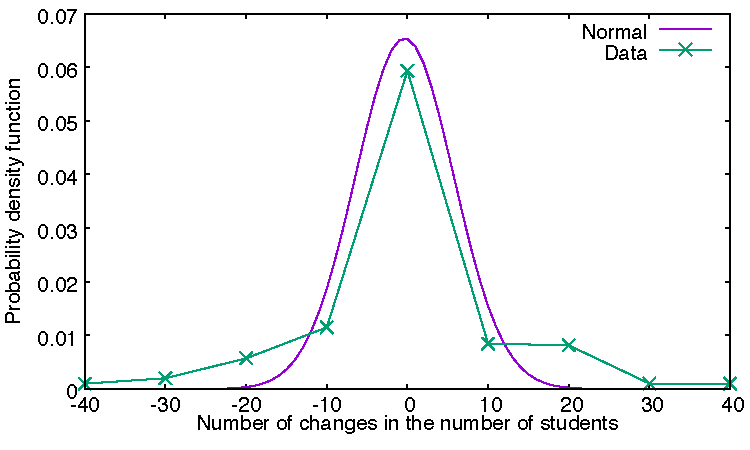
\includegraphics{Figures/perturbationsRoom.pdf}}
    \caption{}
    \label{fig:normalDistStu}
\end{subfigure}
\begin{subfigure}{.5\textwidth}\resizebox{\textwidth}{!}{
    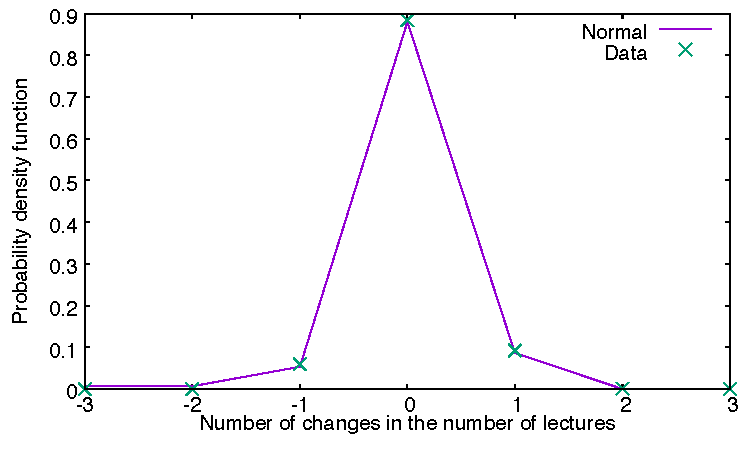
\includegraphics{Figures/perturbationsShift.pdf}}
    \caption{}
    \label{fig:normalDistShift}
\end{subfigure}
\caption{Normal distribution that best fits the data sets of fluctuations in the (a) students enrollments (with mean of -0.3 and standard deviation of 6), and (b) the number of lectures (with mean of 0.04 and standard deviation of 0.45). }
%\vspace{-.5cm}
\end{figure}


The average percentage of disruptions by type is shown in Table~\ref{tab:percentageD}. Note that \textit{time} and \textit{room assignment} represent the probability of a specific lecture to have a preference or a constraint in time or room assignment, respectively. We use these results to randomly generate the number of disruptions of the same type. The disruptions were randomly generated following an uniform distribution. %The developed tool allows the user to specify, in an input file, all the characteristics of the disruption to be generated.% (the file follows the format in Appendix~\ref{app:p1}).The disruption not shown in Table~\ref{tab:percentageD} were not found in the analysis of the timetable for the last 5 years.


 The information shown in Table~\ref{tab:percentageD} is not enough for generating the full set of disruptions. In some cases, it is also necessary to correctly quantify the perturbations in a given lecture/course. This is the case of two specific disruptions: \textit{modify enrollments} and \textit{modify number of lectures}.
 
 For example, when modifying enrollments we need to decide in which lectures the number of students changes (based on the value from Table~\ref{tab:percentageD}) and the actual number to increase/decrease. One could analyze the changes and uniformly select one of these values, since these values are not equiprobable. Therefore, we used the Microsoft Excel Solver~\cite{DBLP:journals/interfaces/FylstraLWW98} to estimate the parameters of a normal distribution that would best fit our data sets. Figure~\ref{fig:normalDistStu} shows the comparison between the closest-fit normal distribution and our data set.
 
 The same process can be applied to find the correct distribution for the disruption \textit{modify number of lectures}. Figure~\ref{fig:normalDistShift} shows the comparison between the closest-fit normal distribution and our data set.
 
 %To sum up, we generate the disruptions based on the history of disruptions of our case study. We generate the disruption randomly following different distributions: uniform and normal. When using the normal distribution, we optimize the parameters to best fit the data. 
 
\subsection{Computational Results}


\subsubsection{Original Problem} In a first approach, we compare the performance of the two different models (proposed in Section 4) when solving the original version of the problem, \emph{i.e.} before disruptions occur. To improve performance, we apply warm-start using the hand-made solution. Note that the hand-made solution is feasible but not optimal. 

Table~\ref{tab:static} shows the results for the different models (\textsc{Boolean} and \textsc{mixed}) when solving the original problem with warm-start. Observe that the \textsc{Boolean} model requires both general (G) and quadratic (Q) constraints. The \textsc{mixed} model requires fewer constraints and variables. In terms of CPU time, the \textsc{Boolean} model is not able to find an optimal solution within the 600 seconds limit. %The \textsc{mixed}  model is the fastest to find the optimal solution for both instances.

It is possible to reduce the size of the problem by reducing the number of students since not all students affect the solution. In this case, the students are used to identify the curricular path. It is natural that groups of students attend the same lectures. Therefore, one does not need to generate constraints for all students. The constraints can be generated only for \textit{distinct} students. In the data sets, around 15\% of all students attend exactly the same lectures. This number is relatively small but allows us to reduce the total number of constraints by 10\% on average for each instance. 

To study the impact of the warm-start strategy in the performance, we run the tests with and without this strategy for the \textsc{mixed} model. The results from \textsc{FALL} and \textsc{SPRING} improve from 1822.57 and 1726.21 to 32.17 and 22.69, respectively.  The version with warm-start is two orders of magnitude faster. The hand-made solution, despite not being optimal, is shown to be a good starting point. 



\begin{table}[t]
\caption{Results for \textsc{Boolean} and \textsc{mixed} models solving the original problem with warm-start, considering general (G) and quadratic (Q) constraints. }
\label{tab:static}
\centering
\resizebox{\textwidth}{!}{%
\begin{tabular}{l|c|c|c|c|c|c|}
\cline{2-5}

                                                        & \multicolumn{2}{c|}{\textsc{FALL}}   & \multicolumn{2}{c|}{\textsc{SPRING}} \\ \cline{2-5} 
                                                         & \textsc{Boolean}     & \textsc{mixed}  & \textsc{Boolean}    & \textsc{mixed}  \\ \hline
%\multicolumn{1}{|c|}{Total CPU Time (s)} &  668.76                & 62.17      &   663.22        & 48.69      \\ \cline{1-5} 
\multicolumn{1}{|l|}{CPU Time (s)} & Time Out                  & 32.17      &    Time Out              & 22.69      \\ \cline{1-5} 
\multicolumn{1}{|l|}{Optimal}                        &   N/A              &  Found     &    N/A               &  Found     \\ \hline
\multicolumn{1}{|l|}{\# Variables}                        &  5269200        &  8487526              &  5255628              &  1668712    \\ \hline
\multicolumn{1}{|l|}{\# Constraints}                        &  5200000 (G) + 5590 (Q)               & 2111238 (G)     & 5187000 (G) + 5460 (Q)     &          1810312 (G)   \\ \hline

\end{tabular}}
\vspace{-.5cm}
\end{table}


\begin{comment}
\centering
\caption{The influence of warm-starting the solver in the CPU time for the \textsc{mixed} model.}
\label{tab:warm}
\begin{tabular}{cc|c|c|}
\cline{3-4}
                                                &        & Warm-start & Without Warm-start \\ \hline
\multicolumn{1}{|c|}{\multirow{2}{*}{CPU Time (s)}} & \textsc{FALL}   & 32.17      & 1822.57            \\ \cline{2-4} 
\multicolumn{1}{|c|}{}                          &  \textsc{SPRING} & 22.69      & 1726.21                   \\ \hline
\end{tabular}
\end{comment}

\vspace{-0.4cm}

\subsubsection{MPP}

The models proposed in this paper were also tested in the presence of disruptions. For each disruption type, 50 different instances were created. Once again and as expected, the \textsc{mixed} model outperforms the \textsc{Boolean} model. For this reason, only the results for the \textsc{mixed} model are shown in Table~\ref{tab:recovery}. In order to improve performance, the warm-start strategy was modified to only add a partial solution (the variables that were affected by the disruption are not added).

The \textsc{SPRING} instance is easier to solve since it has a smaller number of lectures to assign. This fact can be explained by the organization of the curricular plans. %, where the \textsc{SPRING} semester contains the dissertation course which does not have any lectures. 

Let us now analyze the performance. The \textit{modify enrollment} disruption instances are the easiest to be solved. This can be explained by the fact the disruption adds, in general, only a small number of students. The use of slack in the room capacities also contributes to a better performance. This is the only disruption that is able to improve the value of the COM. This disruption also allows reducing the number of students enrolled. \textit{Modify enrollments} is the only disruption to have all instances with a feasible solution. 

The disruptions \textit{invalid time assignment} and \textit{invalid room assignment} cannot lead to a solution with an improved optimization value, given that these disruptions only add new constraints to the problem. The results show that the quality of the solution gets worse with these disruptions. Note that these disruptions may cause the instance to be infeasible. For all instances with feasible solutions, our approach finds optimal solutions. The \textit{invalid time assignment} disruption is the only one to reach the time limit before finding a solution. 

%Globally, one can see that optimizing using COM causes more perturbations in the solution and affects more students. This result confirms the results obtained by Lindahl~\cite{LINDAHL2019}, where is said that performing more perturbation can improve the quality of the solution. Optimizing based the WHD criteria also causes more perturbation but reduces the number of students affected by the change.  





\begin{table}[t]
\caption{Results for the most common disruptions using the \textsc{mixed} model. TO stands for time out, and  $\delta_{COM}$ measures the perturbations in the optimal value. }
\label{tab:recovery}
\centering
\resizebox{\textwidth}{!}{%
\begin{tabular}{c|c|c|c|c|c|c|}
\cline{2-7}
                                                           & \multicolumn{2}{c|}{\textit{Modify Enrollments}}& \multicolumn{2}{c|}{\textit{Invalid  Time}}& \multicolumn{2}{c|}{\textit{Invalid  Room}} \\ \cline{2-7}
                   & \textsc{FALL}                &  \textsc{SPRING}   & \textsc{FALL}                &  \textsc{SPRING}    & \textsc{FALL}                &  \textsc{SPRING}      \\ \hline
 \multicolumn{1}{|c|}{Avg Time (s)}  & 46.2 & 20.65          & TO & TO       &73.36 &60.52                \\ \cline{1-7} 
  \multicolumn{1}{|c|}{Median Time (s)}   & 46.23 & 20.16     & TO &TO     & 72.34 &  59.95                      \\ \cline{1-7} 
 \multicolumn{1}{|c|}{Avg $\delta_{COM}$} & -1 & -1.5       & N/A & N/A     & 0.5&        0           \\ \cline{1-7} 
  \multicolumn{1}{|c|}{COM \% Optimal }   & 100                 &    100  & N/A & N/A  &80 & 90           \\ \cline{1-7} 
  \multicolumn{1}{|c|}{\% Feasible Solution} & 100 & 100   & N/A & N/A                & 80&   90            \\ \hline
\end{tabular}}
\vspace{-.5cm}
\end{table}
\vspace{-0.4cm}


\subsubsection{Incremental Approach for Recovery after Disruption}

The simple recovery process takes too long for the \textit{invalid time assignment} disruption. Therefore, we propose an incremental approach to reduce the search space by splitting the problem into two stages.  A disruption of the type \textit{invalid time assignment} clearly causes a change in the time slots of the lecture. However, it may not be necessary to modify the room assignment. For this reason, we divide the problem into: (i) the problem of assignment of lectures to rooms and (ii) the whole problem. The first stage has to deal with all the constraints relating to time slots, where one has to consider a solution to the problem of assigning rooms to lectures. In this case, the hand-made solution for this sub-problem is added to the model as static. The second stage applies a warm-start with the results of the first stage, possibly improving its quality. This division does not exclude possible solutions since the second stage includes the whole problem again. This decomposition can be changed (\emph{i.e.} start with the problem of assigning lectures to rooms) depending on the disruption since we know beforehand which part of the problem must change. 

Table~\ref{tab:ite} shows the results for the \textit{invalid time assignment} disruption, where one can see that the incremental process is much faster. In this case, the second stage does not improve the quality of the solution. However, it proves the solution to be optimal.

\begin{table}[t]
\centering
\caption{Incremental approach to recover after disruptions of the type \textit{invalid time}. $\delta_{COM}$ measures the change in the optimal value.}
\label{tab:ite}
\begin{tabular}{c|c|c|c|c|}
\cline{2-5}
                                                      & \multicolumn{2}{c|}{\textsc{FALL}} & \multicolumn{2}{c|}{\textsc{SPRING}} \\ \cline{2-5} 
                                                      & Stage 1     & Stage 2     & Stage 1      & Stage 2      \\ \hline
\multicolumn{1}{|c|}{Avg Time (s)}                & 239.02 & 68.67 & 210.68      & 58.4         \\ \hline
\multicolumn{1}{|c|}{Median Time (s)}                 & 282         & 68          & 231.24       & 58           \\ \hline
\multicolumn{1}{|c|}{Avg $\delta_{COM}$ }                     & 2           & 2           & 1            & 1            \\ \hline
\multicolumn{1}{|c|}{\% Feasible Solution} & \multicolumn{2}{c|}{85}   & \multicolumn{2}{c|}{90}     \\ \hline
\end{tabular}
\vspace{-.5cm}
\end{table}


\section{Conclusion and Future Work}\label{sec:con}

This paper discusses the problem of solving university timetabling after some disruption events occur. The integer programming models proposed are able to find a new feasible solution for most common university timetabling disruption scenarios. 
%
To improve the performance, we propose an incremental algorithm that divides the problem into two stages: the problem of assignment of lectures to rooms and the whole problem. The incremental algorithm is able to reduce the size and execution time without losing quality. 
%
Our approaches were successfully evaluated with data sets from \uni. The disruptions were randomly generated with the probability learned from the history of the last five years of timetables. 

%The optimization criterion of the re-solving process can vary from the goal at hand. At IST, if the timetables are not yet in execution, one can take advantage of the disruption to improve the quality of the solution for the students. However, if the disruption occurs during the semester we want to minimize the impact on the students. Our approaches were successfully tested with data sets from the \textit{Taguspark} campus of IST. The disruptions were randomly generated with the probability learn from the history the last five years of timetables in this campus. The models are able to solve the problem, for all disruptions, using different optimization criterion.

%We compared the performance of the different types of models tested: Boolean, Integer and Mixed. The Mixed model was the fastest to solve the data instance since it required fewer constraints and variables. Moreover, non-Boolean encodings were able to avoid quadratic constraints. The results, also shown that using warm-starting techniques in this type of problems provide a significant advantage.  In the case of disruption, the warm-staring procedure only adds a partial and valid solution.

%From the different disruptions tested, the \textit{Modify Enrollments} disruption is the easiest since, in general, it only a small number of students. Moreover, we allow a small percentage of overbooked classrooms. The Modify Enrollments disruption is sometimes able to improve the quality of the overall solution since it also causes a reduction in the number of attending students. To improve the performance, we propose an incremental algorithm which divides the problem into two stages. The first stages focus on solving the only one part of the timetabling problem: the assignment of room to lectures or the assignment of lectures to time slots. The second stage solves the complete problem with the solution from the first part as a starting point. The problem solved in the first stage depends on the disruptions since we know beforehand which part of the problem must change to find a feasible solution. This decomposition reduces the complexity in the first stage and does not remove possible solutions. The results show that this decomposition is able to reduce significantly the CPU time.

As future work, we propose to extend this method in order to benefit from original search data. This way, one could reduce CPU time by avoiding to repeat redundant steps when searching for a new solution.


\newacronym{mpp}{MPP}{Minimal Perturbation Problem}
\newacronym{ilp}{ILP}{Integer Linear Programming}
\newacronym{ist}{IST}{Instituto Superior T\'ecnico}
\newacronym{aoe}{UoAoE}{University of Anywhere on Earth}
\newacronym{cp}{CP}{Constraint Programming}
\newacronym{itc}{ITC}{International Timetabling Competition}
\bibliographystyle{splncs04}\bibliography{cite}
\begin{comment}
\appendix
\section{Disruptions Profile Format}\label{app:p1}
\begin{lstlisting}
Disruptions_type %percentage_of_occurrences

Overlap 11
Preference_Room 13
Invalid_Room 13
Invalid_Time 19
Preference_Time 19
Invalid_Assignment 22
Remove_Room 42
Remove_Room_Day 5 (percentage of closed down rooms)  10 (percentage of
day the room is closed down for)

Disruptions_type %percentage_of_occurrences distribution [mean, standard deviation]

Modify_Enrolments 52 -0.3 6
Modify_N_Lectures 28 0.04 0.45

Disruptions_type #Lectures Average_Length Average_Enrollments

Curriculum 3 3 26
\end{lstlisting}
\end{comment}
\end{document}
